\documentclass[MTech]{iitmdiss}
\usepackage{times}
\usepackage{epsf}
\usepackage{threeparttable}
\usepackage{setspace}
\usepackage{amsmath}
\usepackage{amsthm}
\usepackage{txfonts,pxfonts,amsfonts}
\usepackage{epsfig}	
\usepackage{caption}
\usepackage{subfig}
\usepackage{listings}
\usepackage{epstopdf}
%\usepackage[dvips]{graphicx}
\usepackage{graphicx}
\usepackage{algorithm}
\usepackage{algpseudocode}
%\usepackage{pstricks,pst-node,pst-tree,pstricks-add}
% \usepackage[square,numbers,sort]{natbib}
\usepackage{tikz}
\usetikzlibrary{automata}
\usetikzlibrary{positioning}
\usetikzlibrary{arrows}
\usepackage{boxedminipage}
%\usepackage{biblatex}
\usepackage[square]{natbib}
\usepackage{hyperref}
%\usepackage[hypertex]{hyperref} % hyperlinks for references.
%\usepackage{algorithmic}
\usepackage{multirow}
\usepackage[shortlabels]{enumitem}
\setlist[enumerate]{topsep=10pt}
\usepackage[margin=10pt,
            font=normalsize,
            labelfont=bf,
            labelsep=space,
            position=below]{caption} 
\usepackage{euler} 
%\usepackage{algorithm}
\usepackage{complexity}
\usepackage{booktabs,makecell}
\makeatletter
\newenvironment{breakablealgorithm}
  {% \begin{breakablealgorithm}
   %\begin{center}
     \refstepcounter{algorithm}% New algorithm
     \hrule height.8pt depth0pt \kern2pt% \@fs@pre for \@fs@ruled
     \renewcommand{\caption}[2][\relax]{% Make a new \caption
       {\raggedright\textbf{\ALG@name~\thealgorithm} ##2\par}%
       \ifx\relax##1\relax % #1 is \relax
         \addcontentsline{loa}{algorithm}{\protect\numberline{\thealgorithm}##2}%
       \else % #1 is not \relax
         \addcontentsline{loa}{algorithm}{\protect\numberline{\thealgorithm}##1}%
       \fi
       \kern2pt\hrule\kern2pt
     }
  }{% \end{breakablealgorithm}
     \kern2pt\hrule\relax% \@fs@post for \@fs@ruled
   %\end{center}
  }
\makeatother
%\include{commands}

% Strut macros for skipping spaces above and below text in tables. 
\def\abovestrut#1{\rule[0in]{0in}{#1}\ignorespaces}
\def\belowstrut#1{\rule[-#1]{0in}{#1}\ignorespaces}

\def\abovespace{\abovestrut{0.20in }}
\def\aroundspace{\abovestrut{0.20in}\belowstrut{0.10in}}
\def\belowspace{\belowstrut{0.10in}}
%%%%%%%%%%%%%%%%%%%%%%%%%
\def\thesistitle{Sub-graph Isomorphism in GPU}
\def\thesisauthor{George Joseph}

\begin{document}
\bibliographystyle{iitm}
%%%%%%%%%%%%%%%%%%%%%%%%%%%%%%%%%%%%%%%%%%%%%%%%%%%%%%%%%%%%%%%%%%%%%% 
% Title page

\title{\thesistitle}
\author{\thesisauthor}

\date{May 2017}
\department{Computer Science and Engineering}

%\nocite{*}
\begin{singlespace}
\maketitle 
\end{singlespace} 



%%%%%%%%%%%%%%%%%%%%%%%%%%%%%%%%%%%%%%%%%%%%%%%%%%%%%%%%%%%%%%%%%%%%%%
% Certificate
\certificate
\vspace*{0.5in}
\noindent This is to certify that the thesis entitled {\bf {\thesistitle}}, 
submitted by {\bf {\thesisauthor}}, to the Indian Institute of Technology, 
Madras, for the award of the degree of {\bf Master of Technology}, 
is a bonafide record of the research work carried out by him under my
supervision. The contents of this thesis, in full or in parts, have not been
submitted to any other Institute or University for the award of any degree or diploma.
\vspace*{1.4in}
\hspace*{-0.25in}
\begin{singlespace}
\noindent {\bf Prof.~Rupesh~Nasre} \\
\noindent Research Guide \\ 
\noindent Professor \\
\noindent Dept. of Computer Science and Engineering\\
\noindent IIT-Madras, 600 036 \\
\end{singlespace}
\vspace*{0.20in}
\noindent Place: Chennai\\ 
Date:


%%%%%%%%%%%%%%%%%%%%%%%%%%%%%%%%%%%%%%%%%%%%%%%%%%%%%%%%%%%%%%%%%%%%%%
% Acknowledgements
\acknowledgements
\hspace{10mm}I would like to to express my sincere thanks and deep sense of indebtedness to
my guide Dr. Rupesh Nasre for his guidance and motivation throughout my
work. His inspiring suggestions motivated me to solve problems efficiently. I am
also grateful to my guide also for providing access to the Libra servers without which none of my experiments could have been performed.\par
 \par
I would also thank Vinod Raju, Jithin K M, Nikhil Stephen,Hasit Bhatt,Vivek V P and all my colleagues who always helped me whenever needed in my research. \par
Lastly, I am thankful to god for giving me enough luck to get into IIT Madras and I am thankful to my parents for all the moral support and the amazing
oppurtunities they have given me over the years.


%%%%%%%%%%%%%%%%%%%%%%%%%%%%%%%%%%%%%%%%%%%%%%%%%%%%%%%%%%%%%%%%%%%%%%

%%%%%%%%%%%%%%%%%%%%%%%%%%%%%%%%%%%%%%%%%%%%%%%%%%%%%%%%%%%%%%%%%%%%%%
% Abstract
\abstract


\vspace*{24pt}
In Sub-Graph Isomorphism we are trying to find whether a subgraph of Data Graph is isomorphic to the query graph. Sub-Graph Isomorphism is a NP-Hard problem. Because of the lots of applications of the problem in many Data mining and pattern matching, the problem is well studied and different methods are proposed in the past years. We studied many of the state-of-art techniques used to solve the problem. Then parallelised one of them in GPU. We then tried to solve the dynamic version of the problem. In the dynamic version we remove or add edges on the go and we would like to get the output on the current problem.
\pagebreak
%%%%%%%%%%%%%%%%%%%%%%%%%%%%%%%%%%%%%%%%%%%%%%%%%%%%%%%%%%%%%%%%%
% Table of contents etc.
\begin{singlespace}
\tableofcontents
\thispagestyle{empty}
\listoftables
\addcontentsline{toc}{chapter}{LIST OF TABLES}
\listoffigures
\addcontentsline{toc}{chapter}{LIST OF FIGURES}
\end{singlespace}
%%%%%%%%%%%%%%%%%%%%%%%%%%%%%%%%%%%%%%%%%%%%%%%%%%%%%%%%%%%%%%%%%%%%%%
% Abbreviations
\abbreviations
\noindent 
\begin{tabbing}
xxxxxxxxxxx \= xxxxxxxxxxxxxxxxxxxxxxxxxxxxxxxxxxxxxxxxxxxxxxxx \kill
\textbf{NEC} \> Neighbourhood Equivalence Class \\
\textbf{CVS}   \> Candidate vertex Set \\
\textbf{NDS}   \> Neighbouring Discriminating Substructure \\
\textbf{BFS}   \> Breadth First Search \\

\end{tabbing}



%%%%%%%%%%%%%%%%%%%%%%%%%%%%%%%%%%%%%%%%%%%%%%%%%%%%%%%%%%%%%%%%%%%%%%
%Notation

% \chapter*{\centerline{NOTATION}}
% \addcontentsline{toc}{chapter}{NOTATION}
 
% \begin{singlespace}
% \begin{tabbing}
% xxxxxxxxxxx \= xxxxxxxxxxxxxxxxxxxxxxxxxxxxxxxxxxxxxxxxxxxxxxxx \kill
% \textbf{$r$}  \> Radius, $m$ \\
% \textbf{$\alpha$}  \> Angle of thesis in degrees \\
% \textbf{$\beta$}   \> Flight path in degrees \\
% \end{tabbing}
% \end{singlespace}
 
% \pagebreak
% \clearpage

%The main text will follow from this point so set the page numbering
%to arabic from here on.
\pagenumbering{arabic}

 
%%%%%%%%%%%%%%%%%%%%%%%%%%%%%%%%%%%%%%%%%%%%%%%%%%
 % Chapters.
 \chapter{INTRODUCTION}
\label{chap:intro}
\section{Overview}
Consider that you have pattern and you want to know where all the pattern coming in the data. The pattern can be easily represented as a graph. The actual data can be image video, network of people, etc. The graphs can be used to represent any form of data. The pattern matching has a wide range of application. It is not an easy problem. Since it need a lots of checking at each node. It is similar to placing the pattern at each node in the graph and trying to rotate,flip, etc to find a similar representation. There are lots of possibilities that can match but there may be only small number of actual matching. We need to find them.
\section{Motivation}
As I mentioned before this problem is having lots of applications since the current era is trying to extract lots of features from images, videos,audios,etc using many pattern matching techniques.  Since the problem is NP Hard researchers have focussed on efficiently solving the problem in practice. The numerous cores of GPUs may help us to solve this problem faster. Each node search is independent so they can be done in parallel. This is the  primary motivation on trying to do the sub-graph isomorphism in GPUs. 
\section{Major Contribution}
\begin{itemize}
	\item{Implemented a state-of-Art solution in GPU}
	\item{Dynamic SubGraph Queries are handled in parallel}
\end{itemize}

\section{Organization of Thesis}
	Subgraph Isomorphism chapter \ref{chap:subgraph} discuss the problem and the state-of-art algorithms. A detailed comparison of various algorithms in terms of different pruning techniques is performed.Parallel Implementation \ref{chap:pi} discuss the parallel version of the TurboIso algorithm. Dynamic Operations\ref{chap:dynamic} discuss the implementation of the dynamic version of the problem. The challenges involved in its implementation are discussed in depth.
\chapter{Sub-Graph Isomorphism}
 \label{chap:subgraph}
 \hspace{10mm} In this chapter, the problem statement and various known algorithms for Sub-Graph Isomorphism are studied in great depth. 
 \section{Problem}

\fbox{
  \parbox{\textwidth}{
  \textbf{Input:} A data Graph $D$, and Query Graph $Q$. The graphs $D$ and $Q$ are undirected with nodes and edges having labels.See Figure\ref{fig:graphs}.
  \\
  Graphs given as adjacency list.\\ 
  \textbf{Output:} Give all the matching mapping of each node in $Q$ to node in $D$ \\

}
}\\\\
\begin{figure}

	\begin{minipage}{.5\textwidth}
	\centering
	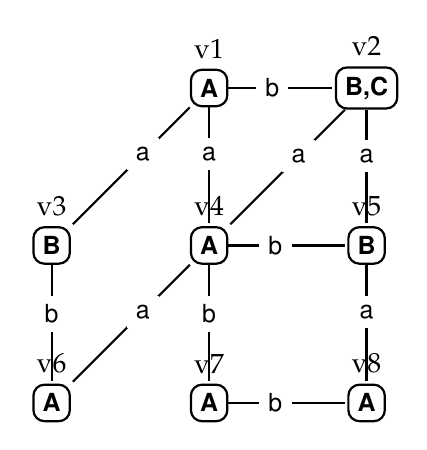
\begin{tikzpicture}[shorten >=1pt,auto,node distance=2cm,
                    thick,main node/.style={rounded corners,draw,font=\sffamily\small\bfseries}]

  \node[main node,label=v1] (1) {A};
  \node[main node,label=v2] (2) [right of=1] {B,C}; 
  \node[main node,label=v4] (4) [below of =1] {A};
  \node[main node,label=v3] (3) [left of=4] {B};
     \node[main node,label=v5] (5) [below of=2] {B};
    \node[main node,label=v6] (6) [below of=3] {A};
    \node[main node,label=v7] (7) [below of=4] {A};
\node[main node,label=v8] (8) [below of=5] {A};
  \path[every node/.style={font=\sffamily\small}]
    (1) edge[] node [minimum width = 1em, fill = white,pos=.25,right] {b} (2)
        edge[] node[minimum width = 1em, fill = white,pos=.25,below left] {a} (3)
        edge[] node[minimum width = 1em, fill = white,pos=.25,below] {a} (4)
    (2) edge[] node [minimum width = 1em, fill = white,pos=.25,below left] {a} (4)
        edge node [minimum width = 1em, fill = white,pos=.25,below] {a} (5)
    (3) edge[] node [minimum width = 1em, fill = white,pos=.25,below] {b} (6)
    (4) edge node [minimum width = 1em, fill = white,pos=.25,below] {b} (7)
    	edge[] node [minimum width = 1em, fill = white,pos=.25,below left] {a} (6) 
    	edge node [minimum width = 1em, fill = white,pos=.25,right] {b} (5) 
    (5) edge node [minimum width = 1em, fill = white,pos=.25,below] {a} (8)
    (7) edge node [minimum width = 1em, fill = white,pos=.25,right] {b} (8);	   
\end{tikzpicture}\\
Data Graph
\end{minipage}
\begin{minipage}{.5\textwidth}
\centering
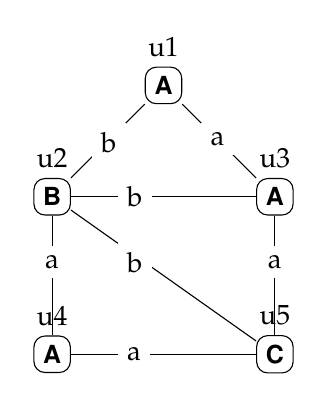
\begin{tikzpicture}[node distance=2cm,node/.style={rounded corners,draw,font=\sffamily\small\bfseries}]
	\node[node,label=u1] (1) {A};
	\node[node,label=u2] (2)[below left of=1] {B};
		\node[node,label=u3] (3)[below right of=1] {A};
		\node[node,label=u4] (4)[below  of=2] {A};
			\node[node,label=u5] (5)[below of=3] {C};
	\path
	(1) edge node [minimum width = 1em, fill = white,pos=.25,below left] {b} (2)
		edge node [minimum width = 1em, fill = white,pos=.25,below right]{a} (3)	
	(2) edge node [minimum width = 1em, fill = white,pos=.25,right]{b} (3)
		edge node [minimum width = 1em, fill = white,pos=.25,below]{a} (4)
		edge node [minimum width = 1em, fill = white,pos=.25,below right]{b} (5)
	(3) edge node [minimum width = 1em, fill = white,pos=.25,below]{a} (5)	
	(4) edge node [minimum width = 1em, fill = white,pos=.25,right]{a} (5);	
							
\end{tikzpicture}
\\ Query Graph
\end{minipage}
\caption{Data and Query Graph}
\label{fig:graphs}
\end{figure}
\hspace{10mm} In Figure \ref{fig:graphs}, 'A' and 'a' represent the node labels and edge labels. A match is present only if the edge labels and node labels are also matched. v1, v2, ... and u1, u2, ... are the node ids. They are used to explain the algorithms discussed below.
\section{Related Work}
\label{sec:rw}
\hspace{10mm}In this section we are discussing various subgraph isomorphism subgraph isomorphism algorithms. Understanding the differences in these algorithms are very crucial.
\subsection{Generic Algorithm}
\label{sec:ga}
	\hspace{10mm}The generic algorithm\cite{GEN} for subgraph isomorphism will help us to study the aspects of state-of-art algorithms in deep. It is presented in Algorithm  \ref{Graph Isomorphism}.\\
\begin{algorithm}[H]
\caption{Subgraph Search}
\label{Graph Isomorphism}
\textbf{Input}: Data Graph $D$,Query Graph $Q$.\\
\textbf{Output}: Mapping of vertices from Q to D.\\
\begin{algorithmic}
 \item \begin{enumerate}
\item for each vertex v of $Q$ 
 \begin{enumerate}
\item C(v)=$FindCandidates$(v,D)
\item If C(v) is empty return 
\end{enumerate}
\item $SUBGRAPHMATCHING$(C,Q,D,$\phi$)
\end{enumerate}
\end{algorithmic}
\textbf{Procedure $SUBGRAPHMATCHING$}:\\
\textbf{Input}: Candidates $C$,Data Graph $D$,Query Graph $Q$ Current Map $M$.\\
\textbf{Output}: Mapping of vertices from Q to D.\\
\begin{algorithmic}
\item \begin{enumerate}
\item if $|M| = |V(q)| $ report M 
\item else
 \begin{enumerate}
\item u=$NextVertex$()
\item $ C_r $ =$RefinedSet$(M,u,C(u))  
\item for each $v \in C_r$ 
 \begin{enumerate}
\item if $IsJoinable$(M,v)
 \begin{enumerate}
\item $UpdateState$(M,v)
\item $SUBGRAPHMATCHING$(q,d,C,M)
\item $RestoreState$(M,v)
\end{enumerate}
\end{enumerate}
\end{enumerate}
\end{enumerate}
\end{algorithmic}
\end{algorithm}
\hspace{10mm}The procedure $FindCandidates$ finds the vertices in datagraph which can be mapped to query vertex. The procedure $NextVertex$ finds the next vertex in querygraph which should be tried to be mapped.

\hspace{10mm}The $RefinedSet$  prunes out some nodes in the candidate set.  The $ IsJoinable$ checks whether the map is right. The $UpdateState$ moves to next state (adds new vertex to map).The $RestoreState$ removes the vertex from map and thus restores the state.

\hspace{10mm} If you consider the graphs in Figure \ref{fig:graphs}. $C(u1)=\{v1,v6,v7,v8\}$ pruned by node label and degree. Similiarly $C(u4)=\{v1,v6,v7,v8\}$ and $C(u2)=\{v3,v2,v5\}$. Procedure $NextGraph$ will give the vertices on query graph in some order like $\{u1,u2,u3,u4,u5\}$. It can be even $\{ u1, u3,u4,u2,u5\}$. Once $ u1$ is mapped to $v1$,the procedure $RefinedSet$ will remove $v1$ from $C(u4)$. If Map has these values $\{(u1,v1)\}$,$NextGraph$ returned $u2$ , $RefinedSet$ returned $\{v3,v2,v5\}$ and current $v$ is $v5$ then procedure $IsJoinable$ check whether there is an edge between $v1 $ and $v5$ like the one between $u1$ and $u2$.  
\subsection{Ullmann Algorithm}
\label{sec:ullmann}
\hspace{10mm}This algorithm\cite{Ull} is simple.The $FindCandidates$ finds same degree nodes. The $NextVertex$ takes the next node in input.The $RefinedSet$ removes nodes already mapped.  The procedure $ IsJoinable$ iterates over the neighborhood and checks if corresponding edge exists. The $UpdateState$ and $RestoreState$ adds and removes the vertex from map respectively.
\subsection{VF2 Algorithm}
\label{sec:vf2}
\hspace{10mm}VF2 algorithm was proposed in \cite{VF2}.The $NextVertex$ takes the next connected vertex. The $RefinedSet$ uses these rules
 \begin{enumerate}
 \item Prune out v if not connected from already mapped vertices.
 \item The count of unmatched vertices of neighbors of v in $Q$ must be greater than unmatched vertices of neighbors of u in $D$
 \item The count of neighbors of v who are not neighbors of mapped nodes and not mapped nodes in $Q$ must be greater than neighbors of u who are not neighbors of mapped nodes and not mapped nodes in $D$
 \end{enumerate}
\subsection{QucikSi Algorithm}
\label{sec:qsi}
\hspace{10mm}QuickSi algorithm was proposed in \cite{QSI}.The $NextVertex$ takes vertices in the most infrequent vertex first order.The $RefinedSet$ uses connectivity to mapped vertices to prune.The $RefinedSet$ only iterates over mapped adjacent vertices.
\subsection{GADDI Algorithm}
\label{sec:gaddi}
	\hspace{10mm}GADDI was proposed in \cite{GAD}. They use the neighboring discriminating substructure(NDS).$\Delta_{NDS}(u,v,P)$ is the number of occurrences of P in induced subgraph $N_k(v) \cap N_k(u)$. $N_k(u) $ is the graph having all the edges in k distance from u. A matrix L is created such that each row corresponds to an induced graph g and each column represent a pattern. See the NDS calculation in Figure \ref{fig:gaddi}. The dark lines represent the $N_k(v1) \cap N_k(v3)$ with k=2, ie., nodes and edges at a distance of at most 2 from both the vertices $v1$ and $v2$. The $NextVertex$ takes the one next in the DFS Tree from  the vertex. The $RefinedSet$ prune based on these conditions.
\\	\hspace{10mm}If for each $u^{'} \in N_{k}(u)$ there is no data vertex $v^{'} \in N_{k}(v)$ having
	\begin{enumerate}
 \item $L(u^{'}) \subseteq L(v^{'})$ 
 \item The shortest distance between $v^{'}$ and $v$ must be greater than or equal to distance between $u$ and $u^{'}$ .
 \end{enumerate}
 \begin{figure}
	\begin{minipage}{.6\textwidth}
	\centering
	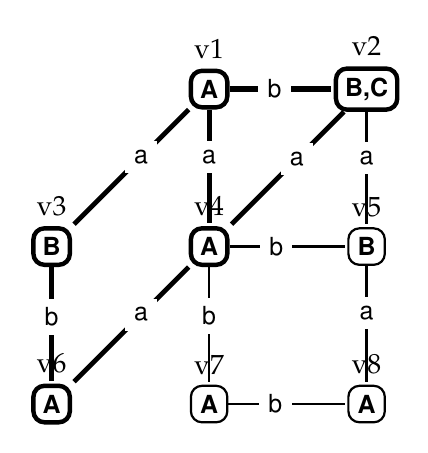
\begin{tikzpicture}[shorten >=1pt,auto,node distance=2cm,
                    thick,main node/.style={rounded corners,draw,font=\sffamily\small\bfseries}]

  \node[line width=1.6pt,main node,label=v1] (1) {A};
  \node[line width=1.6pt,main node,label=v2] (2) [right of=1] {B,C}; 
  \node[line width=1.6pt,main node,label=v4] (4) [below of =1] {A};
  \node[line width=1.6pt,main node,label=v3] (3) [left of=4] {B};
     \node[main node,label=v5] (5) [below of=2] {B};
    \node[line width=1.6pt,main node,label=v6] (6) [below of=3] {A};
    \node[main node,label=v7] (7) [below of=4] {A};
\node[main node,label=v8] (8) [below of=5] {A};
  \path[every node/.style={font=\sffamily\small}]
    (1) edge[line width=.7mm] node [minimum width = 1em, fill = white,pos=.25,right] {b} (2)
        edge[line width=.6mm] node[minimum width = 1em, fill = white,pos=.25,below left] {a} (3)
        edge[line width=.65mm] node[minimum width = 1em, fill = white,pos=.25,below] {a} (4)
    (2) edge[line width=.6mm] node [minimum width = 1em, fill = white,pos=.25,below left] {a} (4)
        edge node [minimum width = 1em, fill = white,pos=.25,below] {a} (5)
    (3) edge[line width=.65mm] node [minimum width = 1em, fill = white,pos=.25,below] {b} (6)
    (4) edge node [minimum width = 1em, fill = white,pos=.25,below] {b} (7)
    	edge[line width=.6mm] node [minimum width = 1em, fill = white,pos=.25,below left] {a} (6) 
    	edge node [minimum width = 1em, fill = white,pos=.25,right] {b} (5) 
    (5) edge node [minimum width = 1em, fill = white,pos=.25,below] {a} (8)
    (7) edge node [minimum width = 1em, fill = white,pos=.25,right] {b} (8);	   
\end{tikzpicture}\\
$ \Delta_{NDS}(v1,v3,P1)=6 , \Delta_{NDS}(v1,v3,P2)=24 ~,~\Delta_{NDS}(v1,v3,P3)=12$
\end{minipage}
\begin{minipage}{.35\textwidth}
\centering
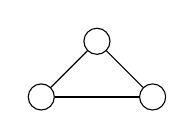
\begin{tikzpicture}[node distance=1cm]
\node[circle,draw] (1)[]{};
\node[circle,draw] (2)[below left  of=1]{};
\node[circle,draw] (3)[below right  of=1]{};
\path
	(1) edge node{} (2)
		 edge node{} (3)
	(2) edge node{} (3);	
\end{tikzpicture}
\\ P1\\ \hfill \\
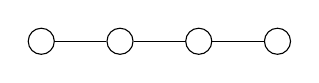
\begin{tikzpicture}[node distance=1cm]
\node[circle,draw] (1)[]{};
\node[circle,draw] (2)[right of=1]{};
\node[circle,draw] (3)[right of=2]{};
\node[circle,draw] (4)[right of=3]{};
\path
	(1) edge node{} (2)
	(2) edge node{} (3)
	(3) edge node{} (4);	
\end{tikzpicture}
\\ P2\\ \hfill \\
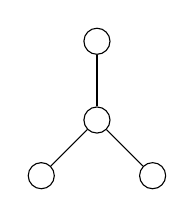
\begin{tikzpicture}[node distance=1cm]
\node[circle,draw] (4)[]{};
\node[circle,draw] (1)[below of =4]{};
\node[circle,draw] (2)[below left  of=1]{};
\node[circle,draw] (3)[below right  of=1]{};

\path
	(1) edge node{} (2)
		 edge node{} (3)
	(4) edge node{} (1);	
\end{tikzpicture}
\\ P3
\end{minipage}
\caption{GADDI NDS Calculation}
\label{fig:gaddi}
\end{figure}
\hspace{10mm}The triangles(P1) present in the $N_k(v1) \cap N_k(v3)$ is 6. The vertices $v1$, $v2$ and $v4$ make the 6 traingles(6 permutation of vertices). The number of lines of length 3(p2) present in the graph is 24. The vertices $v1$, $v2$, $v4$ and $v6$ makes one of the 24 lines. The stars(P3) present are at vertices $v1$ and $v4$. The different combinations gives 12 possibilities.
 \subsection{GraphQL Algorithm}
 \label{sec:gql}
\hspace{10mm}The GraphWl was proposed in \cite{GQL}. They use neighborhood signatures. The neighbor of the vertex is encoded as the collection of labels of its neighbors.  The $RefinedSet$  pruning is based on this signature. This is a one hop signature. For example the $sig(u1) =\{B,A\}$ in Figure \ref{fig:graphs}.

\subsection{SPath Algorithm}
\label{sec:spath}
\hspace{10mm}The SPath Algorithm was proposed in \cite{SPA}. They use signatures till k hop. They store the signature in the form $(d,l,c)$ where d is distance to the neighbor, l the label,c the  count.The $RefinedSet$  pruning is based on these signatures.For example the $sig(u1,2) = \{(1,B,1),(1,A,1),(2,A,1),(2,C,1)\}$ in Figure \ref{fig:graphs}.
\subsection{STWig Algorithm}
\label{sec:stwig}
	\hspace{10mm}The STWig Algorithm was proposed in \cite{STWig}. Here the query graph is divided into smaller graphs. These smaller graphs are searched in the data graph first. Their results are combined to get the final result. The graphs are divided such that the root of $g_j$ must be of the children of any of the graphs $g_i$ such that $i<j$. All STWigs are two level trees. See Figure \ref{fig:stwig} for a random STWigs generated for query graph in Figure \ref{fig:graphs}. There is no constraint in number of children allowed. So there are many decomposition for a graph.
	 \par The candidates can be started from the least frequent pattern and then building up. The splitting of the graphs,matching the small STWigs and then combining can be done in GPU. But the combining of STWig results in the troublesome task. This can lead to the need of large amount of memory too since the candidate set can increase exponentialy.
	\begin{figure}[h]
 \centering
%\centering
\begin{minipage}{.24\textwidth}
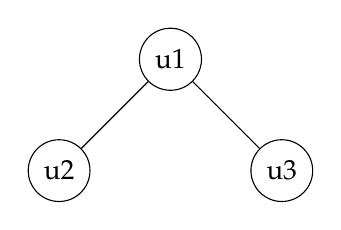
\begin{tikzpicture}[node distance=2cm]
\node[circle,draw] (1)[]{u1};
\node[circle,draw] (2)[below left  of=1]{u2};
\node[circle,draw] (3)[below right  of=1]{u3};
\path
	(1) edge node{} (2)
		 edge node{} (3);	
\end{tikzpicture}
\end{minipage}
\begin{minipage}{.24\textwidth}
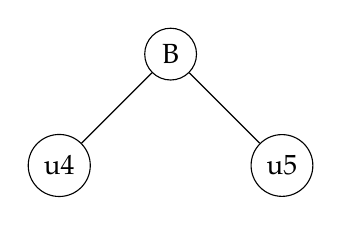
\begin{tikzpicture}[node distance=2cm]
\node[circle,draw] (1)[]{B};
\node[circle,draw] (2)[below left  of=1]{u4};
\node[circle,draw] (3)[below right  of=1]{u5};
\path
	(1) edge node{} (2)
		 edge node{} (3);	
\end{tikzpicture}
\end{minipage}
\begin{minipage}{.24\textwidth}
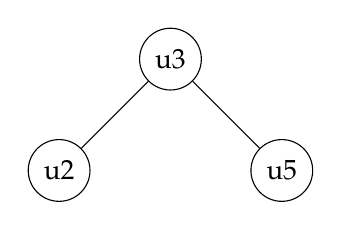
\begin{tikzpicture}[node distance=2cm]
\node[circle,draw] (1)[]{u3};
\node[circle,draw] (2)[below left  of=1]{u2};
\node[circle,draw] (3)[below right  of=1]{u5};
\path
	(1) edge node{} (2)
		 edge node{} (3);	
\end{tikzpicture}
\end{minipage}
\begin{minipage}{.24\textwidth}
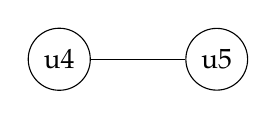
\begin{tikzpicture}[node distance=2cm]
\node[circle,draw] (1)[]{u5};
\node[circle,draw] (2)[ left  of=1]{u4};
\path
	(1) edge node{} (2)	;
\end{tikzpicture}
\end{minipage}
 \caption{STWig Decomposition}
 \label{fig:stwig}
\end{figure}
\hspace{10mm} 
\section{Implemented Algorithm}
\label{sec:implementation}
\subsection{TurboIso}
\label{sec:tiso}
	\hspace{10mm}It was proposed in \cite{Turbosio}.$Turbo_{iso}$ uses neighborhood equivalence class(NEC). Here they make a tree out of the query graph. In this tree they create the NEC. Each node will be part of a unique NEC. Later this tree is searched in the data graph. Then the graph edges are checked. 
	
	\begin{figure}[h]
 \centering
%\centering
\begin{minipage}{.6\textwidth}

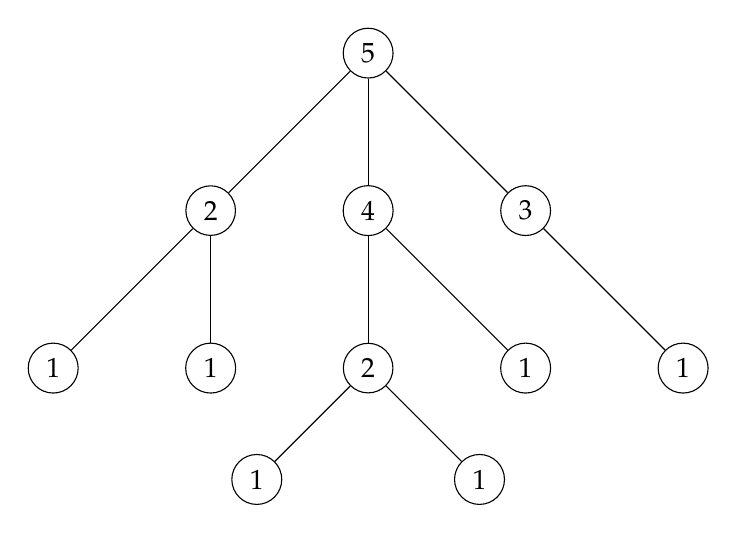
\begin{tikzpicture}[node distance=2cm]
\node[circle,draw] (1)[]{5};
\node[circle,draw] (3)[below of=1]{4};
\node[circle,draw] (2)[left of=3]{2};

\node[circle,draw] (4)[ right of=3]{3};
\node[circle,draw] (5)[below of=2]{1};
\node[circle,draw] (6)[left of=5]{1};
\node[circle,draw] (7)[below of=3]{2};
\node[circle,draw] (8)[right of=7]{1};
\node[circle,draw] (9)[right of=8]{1};
\node[circle,draw] (10)[below left of=7]{1};
\node[circle,draw] (11)[below right of=7]{1};
\path
	(1) edge node{} (2)
		 edge node{} (3)
		 edge node{} (4)
	(2) edge node{} (5)
		edge node{} (6)
	(3) edge node{} (7)
		edge node{} (8)
	(4) edge node{} (9)
	(7) edge node{} (10)
		edge node{} (11);	
\end{tikzpicture}
\end{minipage}
\begin{minipage}{.2\textwidth}
\centering
NEC 4\hfill \\
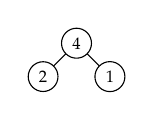
\begin{tikzpicture}[scale=0.1,every node/.style={scale=0.6}]

\node[circle,draw] (2){4};
\node[circle,draw] (3)[below left of=2]{2};
\node[circle,draw] (4)[below right of=2]{1};
\path
	(2)	 edge node{} (3)
		 edge node{} (4);
\end{tikzpicture}
\\NEC 3 \hfill \\
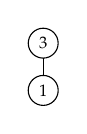
\begin{tikzpicture}[scale=0.1,every node/.style={scale=0.6}]

\node[circle,draw] (1)[]{3};
\node[circle,draw] (3)[below of=1]{1};
\path
	
	(1) edge node{} (3);
\end{tikzpicture}
\\NEC 2\hfill \\
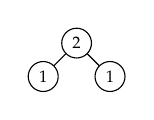
\begin{tikzpicture}[scale=0.1,every node/.style={scale=0.6}]

\node[circle,draw] (1)[]{2};
\node[circle,draw] (2)[below left of=1]{1};
\node[circle,draw] (3)[below right of=1]{1};

\path
	
	(1) edge node{} (3)
		edge node{} (2);
\end{tikzpicture}
\\NEC 5 \hfill \\
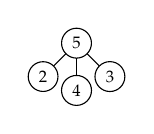
\begin{tikzpicture}[scale=0.1,every node/.style={scale=0.6}]

\node[circle,draw] (1)[]{5};
\node[circle,draw] (2)[below left of=1]{2};
\node[circle,draw] (4)[below of=1]{4};
\node[circle,draw] (3)[below right of=1]{3};

\path
	
	(1) edge node{} (3)
		edge node{} (4)
		edge node{} (2);
\end{tikzpicture}
\\Classes
\end{minipage}

 \caption{NEC Numbering}
 \label{fig:nec}
\end{figure}


\begin{algorithm}[H]

\caption{NEC creation}
%\label{Graph Isomorphism}
\textbf{Input}: Data Graph $D$,Query Graph $Q$.\\
\textbf{Output}: Mapping of vertices from Q to D.\\
\begin{algorithmic}
\item \begin{enumerate}
\item The leaf nodes are given NEC 1
\item for each level upward
\begin{enumerate}
\item Each new neighborhood will get a new NEC
\end{enumerate}
\end{enumerate}
\end{algorithmic}
\label{alg:nec}
\end{algorithm}
\hspace{10mm} In figure \ref{fig:nec}, the leaf nodes are given the NEC 1. Then the algorithm \ref{alg:nec} moves upward each level. In the succeeding level it finds two more classes NEC 2 and NEC 3. The numbering are given a sequential order. In the next level it find the NEC 5. The corresponding NEC's can be seen on the right of the image. Then CVS for each NEC is found in the data graph. Then for each combination the actual graph is tested for a match. 

\hspace{10mm} The CVS is the collection of all matching vertices of data graph for each NEC. This is found out by checking the existence of the NEC children at each data graph node. Each node in data graph is given a NEC 1. Then each higher NECs are checked. After that all possible combinations are checked for existence of the graph. If a match is found, it is printed.


\subsection{Inferences}
\label{sec:findings}
	\hspace{10mm}All of the above algorithms tried to decrease the total candidate vertices set(CVS) for a vertex in query graph. The permutation and combination of these vertices will result in the final answer. More the CVS, more will be the combinations. Since the answer requires all possible permutations we can't avoid this calculation. So we need to prune out the false candidate as early as possible. This is the reason why intermediate pruning steps are added in $UpdateState$ also. The neighborhood signature is the way seen so far to prune the CVS initially better.


\chapter{Parallel Implementation}
 \label{chap:pi}
 \section{Introduction}
\hspace{10mm}In the parallel implementation the unique NEC numbering, CVS generation in data graph, and checking whether the query graph exists in the sub-graph and the combination generation are done in GPU.

\section{Algorithm}
 \label{sec:al}
 
\begin{breakablealgorithm}[H]
\caption{Parallel $Turbo_{iso}$}
%\label{Graph Isomorphism}
\textbf{Procedure}: NECGen()\\
Parallel NEC generation on each node.\\
\textbf{Input}: Query Graph $Q$.\\
\textbf{Output}: NEC.\\
\begin{algorithmic}
\item \begin{enumerate}
\item repeat until all nodes got NEC
\item Run parallel on all nodes
\begin{enumerate}
\item running on node v
\item iterate over all neighbors of vertex v
\item \hspace{10mm}if not all neighbors have NEC return
\item find the hash of neighborhood.set its hash location to 1.
\end{enumerate}
\item assign unique numbering to all 1's in the hash array
\item Run parallel on all nodes
\begin{enumerate}
\item running on node v
\item iterate over all neighbors of vertex v
\item \hspace{10mm}if not all neighbors have NEC return
\item find the hash of neighborhood.Find the unique NEC in hash location
\item assign it to the vertex
\end{enumerate}
\end{enumerate}
\end{algorithmic}
\textbf{Procedure}: CVSGen()\\
Parallel CVS generation for each NEC.\\
\textbf{Input}: Data Graph $Q$,NEC.\\
\textbf{Output}: CVS.\\
\begin{algorithmic}
\item \begin{enumerate}
\item all nodes in data graph is in NEC 1
\item for each NEC from 2 to last
\item Run parallel on all nodes
\begin{enumerate}
\item running on node v
\item iterate over all neighbors of vertex v.
\item \hspace{10mm}check the existence of the neighborhood of NEC on the node v.
\item \hspace{10mm}if found set the flag 1.
\end{enumerate}
\end{enumerate}
\end{algorithmic}
\textbf{Procedure}: PermandComb()\\
Parallelly check all possible permutations and combinations.\\
\textbf{Input}: Data Graph $D$, Query Graph $Q$, Current vertex index(i),Possibilities(P),Maximum Possibilities(MP)\\
\textbf{Output}: Mapping of nodes from query graph to data graph.\\
\begin{algorithmic}
\item \begin{enumerate}
\item if i= $|V(q)|$
\item \hspace{10mm}Report all values in P and return
\item else
 \begin{enumerate}
\item find u,the NEC of the vertex
\item Multiply P with CVSGen(u)
\item while $P >= MP$
 \begin{enumerate}
\item call CheckMap() on MP elements of P
\item call Exclusive-scan on Checkmap output
\item Save valid possibilities to newP 
\item P-=MP (numbers)
\end{enumerate}
\item move newP to P.
\end{enumerate}
\end{enumerate}
\end{algorithmic}
\textbf{Procedure}: CheckMap()\\
Parallel check of existence of query graph.\\
\textbf{Input}: Data Graph $D$,Map m,Query Graph $Q$,till vertex $v$ in query graph.\\
\textbf{Output}: true/false.\\
\begin{algorithmic}
\item \begin{enumerate}
\item running on all nodes u if $u<=v$.
\item iterate over all neighbors of vertex u.
\item \hspace{10mm}check the existence of all edges in data graph corresponding to one in query graph.
\item \hspace{10mm}if not all edges present set false.
\end{enumerate}

\end{algorithmic}
\end{breakablealgorithm}
\par The procedure $NECGen$ gives unique ids to one tree in the query graph similar to Figure 4. We do a level order traversal on the tree. So at some nodes all its children may not have NEC given we process those nodes in the next iterations. The step 2 finds the neighborhoods that can be processed at the current iteration and finds a hash of the neighborhood. To these unique hashes we assign numbering by SCAN algorithm. Then these numbering are assigned back to each nodes.
\par The procedure $CVSGen $ finds the candidates for a particular NEC. They check on each node on data graph and checks the neighboring nodes for matching neighbors of the particular NEC in query graph.
\par The procedure $PermandComb$ finds all possibilities of the query graph. For each vertex of query graph it finds all possibilities(current possibilities x CvsGen(u)). If the possibilities is more than we can store(MP), $CheckMap$ is called on all current possibilities and the wrong ones are removed. This will make the P $<$MP.  At last when i= $|V(q)|$,  P has all valid possibilities. The procedure $CheckMap$ checks the existence of non tree edges in the current 	mapping. If $CheckMap$ returns true it is reported as a correct mapping.
\begin{figure}[h!]
 \begin{minipage}{.3\textwidth}
 \centering
  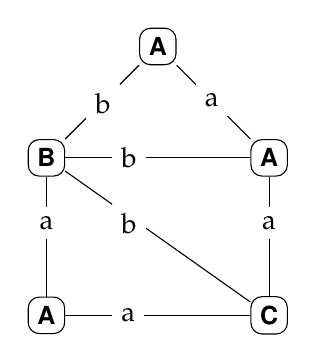
\begin{tikzpicture}[node distance=2cm,node/.style={rounded corners,draw,font=\sffamily\small\bfseries}]
	\node[node] (1) {A};
	\node[node] (2)[below left of=1] {B};
		\node[node] (3)[below right of=1] {A};
		\node[node] (4)[below  of=2] {A};
			\node[node] (5)[below of=3] {C};
	\path
	(1) edge node [minimum width = 1em, fill = white,pos=.25,below left] {b} (2)
		edge node [minimum width = 1em, fill = white,pos=.25,below right]{a} (3)	
	(2) edge node [minimum width = 1em, fill = white,pos=.25,right]{b} (3)
		edge node [minimum width = 1em, fill = white,pos=.25,below]{a} (4)
		edge node [minimum width = 1em, fill = white,pos=.25,below right]{b} (5)
	(3) edge node [minimum width = 1em, fill = white,pos=.25,below]{a} (5)	
	(4) edge node [minimum width = 1em, fill = white,pos=.25,right]{a} (5);	
							
\end{tikzpicture}
\\\textbf{Step 1}
\end{minipage}
 \begin{minipage}{.3\textwidth}
	 \centering
	 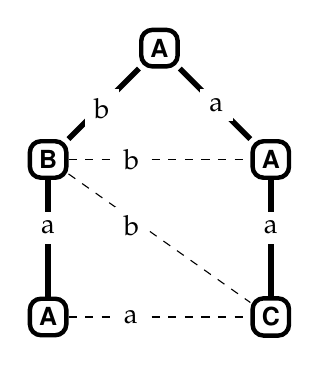
\begin{tikzpicture}[node distance=2cm,node/.style={rounded corners,draw,font=\sffamily\small\bfseries}]
	\node[node,line width=1.6pt] (1) {A};
	\node[node,line width=1.6pt] (2)[below left of=1] {B};
		\node[node,line width=1.6pt] (3)[below right of=1] {A};
		\node[node,line width=1.6pt] (4)[below  of=2] {A};
			\node[node,line width=1.6pt] (5)[below of=3] {C};
	\path
	(1) edge[line width=.7mm] node [minimum width = 1em, fill = white,pos=.25,below left] {b} (2)
		edge[line width=.7mm] node [minimum width = 1em, fill = white,pos=.25,below right]{a} (3)	
	(2) edge[dashed] node [minimum width = 1em, fill = white,pos=.25,right]{b} (3)
		edge[line width=.7mm] node [minimum width = 1em, fill = white,pos=.25,below]{a} (4)
		edge[dashed] node [minimum width = 1em, fill = white,pos=.25,below right]{b} (5)
	(3) edge[line width=.7mm] node [minimum width = 1em, fill = white,pos=.25,below]{a} (5)	
	(4) edge[dashed] node [minimum width = 1em, fill = white,pos=.25,right]{a} (5);	
							
\end{tikzpicture}
\\\textbf{Step 2}
\end{minipage}
\begin{minipage}{.3\textwidth}
	 \centering
	 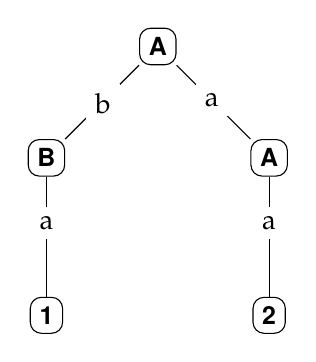
\begin{tikzpicture}[node distance=2cm,node/.style={rounded corners,draw,font=\sffamily\small\bfseries}]
	\node[node] (1) {A};
	\node[node] (2)[below left of=1] {B};
		\node[node] (3)[below right of=1] {A};
		\node[node] (4)[below  of=2] {1};
			\node[node] (5)[below of=3] {2};
	\path
	(1) edge[] node [minimum width = 1em, fill = white,pos=.25,below left] {b} (2)
		edge[] node [minimum width = 1em, fill = white,pos=.25,below right]{a} (3)	
	(2) edge[] node [minimum width = 1em, fill = white,pos=.25,below]{a} (4)
	(3) edge[] node [minimum width = 1em, fill = white,pos=.25,below]{a} (5);							
\end{tikzpicture}
\\\textbf{Step 3}
\end{minipage}\\
\vspace{5mm}
\begin{minipage}{.3\textwidth}
	 \centering
	 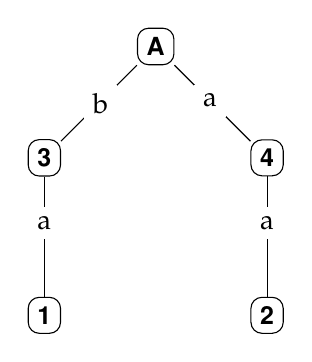
\begin{tikzpicture}[node distance=2cm,node/.style={rounded corners,draw,font=\sffamily\small\bfseries}]
	\node[node] (1) {A};
	\node[node] (2)[below left of=1] {3};
		\node[node] (3)[below right of=1] {4};
		\node[node] (4)[below  of=2] {1};
			\node[node] (5)[below of=3] {2};
	\path
	(1) edge[] node [minimum width = 1em, fill = white,pos=.25,below left] {b} (2)
		edge[] node [minimum width = 1em, fill = white,pos=.25,below right]{a} (3)	
	(2) edge[] node [minimum width = 1em, fill = white,pos=.25,below]{a} (4)
	(3) edge[] node [minimum width = 1em, fill = white,pos=.25,below]{a} (5);							
\end{tikzpicture}
\\\textbf{Step 4}
\end{minipage}
\begin{minipage}{.3\textwidth}
	 \centering
	 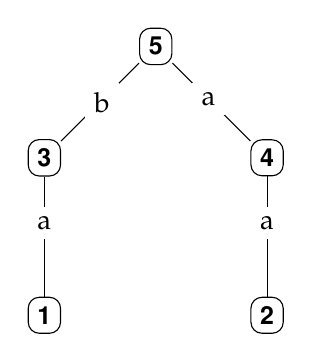
\begin{tikzpicture}[node distance=2cm,node/.style={rounded corners,draw,font=\sffamily\small\bfseries}]
	\node[node] (1) {5};
	\node[node] (2)[below left of=1] {3};
		\node[node] (3)[below right of=1] {4};
		\node[node] (4)[below  of=2] {1};
			\node[node] (5)[below of=3] {2};
	\path
	(1) edge[] node [minimum width = 1em, fill = white,pos=.25,below left] {b} (2)
		edge[] node [minimum width = 1em, fill = white,pos=.25,below right]{a} (3)	
	(2) edge[] node [minimum width = 1em, fill = white,pos=.25,below]{a} (4)
	(3) edge[] node [minimum width = 1em, fill = white,pos=.25,below]{a} (5);							
\end{tikzpicture}
\\\textbf{Step 5}
\end{minipage}
\begin{minipage}{.3\textwidth}
	 \centering
	 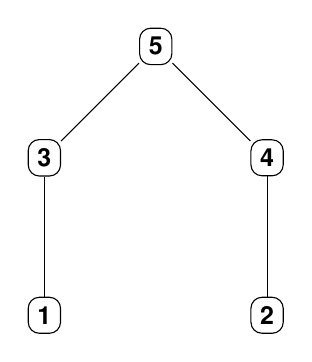
\begin{tikzpicture}[node distance=2cm,node/.style={rounded corners,draw,font=\sffamily\small\bfseries}]
	\node[node] (1) {5};
	\node[node] (2)[below left of=1] {3};
		\node[node] (3)[below right of=1] {4};
		\node[node] (4)[below  of=2] {1};
			\node[node] (5)[below of=3] {2};
	\path
	(1) edge[] node [] {} (2)
		edge[] node []{} (3)	
	(2) edge[] node []{} (4)
	(3) edge[] node []{} (5);							
\end{tikzpicture}
\\\textbf{Step 6}
\end{minipage}\\
\vspace{5mm}
\begin{minipage}{.3\textwidth}
\centering
\hfill \\

\begin{tikzpicture}[node distance=2cm,node/.style={rounded corners,draw,font=\sffamily\small\bfseries}]
\node[node,label=NEC 1] (2){A};
\end{tikzpicture}\\
\hfill \\
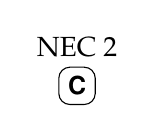
\begin{tikzpicture}[node distance=2cm,node/.style={rounded corners,draw,font=\sffamily\small\bfseries}]
\node[node,label=NEC 2] (2){C};
\end{tikzpicture}\\
\hfill \\
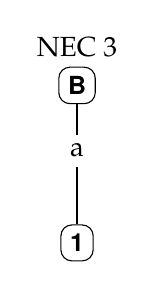
\begin{tikzpicture}[node distance=2cm,node/.style={rounded corners,draw,font=\sffamily\small\bfseries}]

\node[node,label=NEC 3] (2){B};
\node[node] (3)[below of=2]{1};
\path
	(2)	 edge node[minimum width = 1em, fill = white,pos=.25,below ] {a} (3);
\end{tikzpicture}
\end{minipage}
\begin{minipage}{.3\textwidth}
\centering
\hfill \\
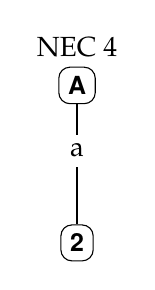
\begin{tikzpicture}[node distance=2cm,node/.style={rounded corners,draw,font=\sffamily\small\bfseries}]

\node[node,label=NEC 4] (2){A};
\node[node] (3)[below of=2]{2};
\path
	(2)	 edge node[minimum width = 1em, fill = white,pos=.25,below ] {a} (3);
\end{tikzpicture}
\hfill \\
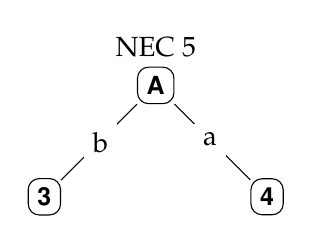
\begin{tikzpicture}[node distance=2cm,node/.style={rounded corners,draw,font=\sffamily\small\bfseries}]

\node[node,label=NEC 5] (2){A};
\node[node] (3)[below left of=2]{3};
\node[node] (4)[below right of=2]{4};
\path
	(2)	 edge node[minimum width = 1em, fill = white,pos=.25,below left] {b} (3)
		 edge node[minimum width = 1em, fill = white,pos=.25,below right] {a} (4);
\end{tikzpicture}
\\Classes
\end{minipage}
 \caption{Algorithm Query Graph Processing}
 \label{fig:working}
\end{figure}
 \par In the figure \ref{fig:working} the NEC's in query graph are detected. The first step is the finding of tree in the query graph. The bold lines in the image shows the selected tree in the query graph. In the next step the leaf nodes are given unique NEC's according to the node label. Then at each step the parent nodes whose all children has NEC defined, is given new NEC's. See the figure \ref{fig:working} and the NEC classes are given in the end. The NEC's are taking care of the edge labels so they are no longer required in the graph. 
\begin{figure}[h!]
\begin{minipage}{.4\textwidth}
	\centering
	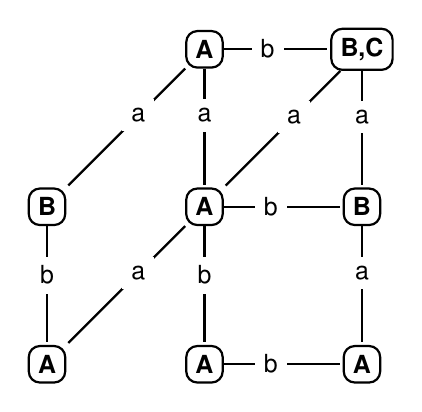
\begin{tikzpicture}[shorten >=1pt,auto,node distance=2cm,
                    thick,main node/.style={rounded corners,draw,font=\sffamily\small\bfseries}]

  \node[main node] (1) {A};
  \node[main node] (2) [right of=1] {B,C}; 
  \node[main node] (4) [below of =1] {A};
  \node[main node] (3) [left of=4] {B};
     \node[main node] (5) [below of=2] {B};
    \node[main node] (6) [below of=3] {A};
    \node[main node] (7) [below of=4] {A};
\node[main node] (8) [below of=5] {A};
  \path[every node/.style={font=\sffamily\small}]
    (1) edge[] node [minimum width = 1em, fill = white,pos=.25,right] {b} (2)
        edge[] node[minimum width = 1em, fill = white,pos=.25,below left] {a} (3)
        edge[] node[minimum width = 1em, fill = white,pos=.25,below] {a} (4)
    (2) edge[] node [minimum width = 1em, fill = white,pos=.25,below left] {a} (4)
        edge node [minimum width = 1em, fill = white,pos=.25,below] {a} (5)
    (3) edge[] node [minimum width = 1em, fill = white,pos=.25,below] {b} (6)
    (4) edge node [minimum width = 1em, fill = white,pos=.25,below] {b} (7)
    	edge[] node [minimum width = 1em, fill = white,pos=.25,below left] {a} (6) 
    	edge node [minimum width = 1em, fill = white,pos=.25,right] {b} (5) 
    (5) edge node [minimum width = 1em, fill = white,pos=.25,below] {a} (8)
    (7) edge node [minimum width = 1em, fill = white,pos=.25,right] {b} (8);	   
\end{tikzpicture}
\\\textbf{Step 1}
\end{minipage}
\begin{minipage}{.4\textwidth}
	\centering
	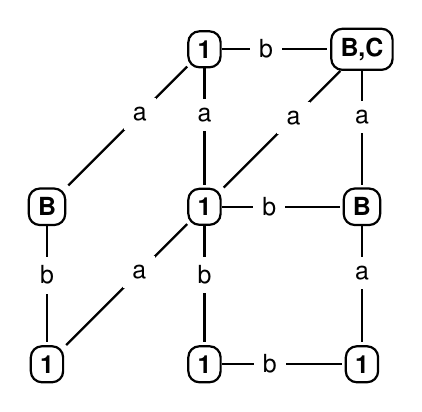
\begin{tikzpicture}[shorten >=1pt,auto,node distance=2cm,
                    thick,main node/.style={rounded corners,draw,font=\sffamily\small\bfseries}]

  \node[main node] (1) {1};
  \node[main node] (2) [right of=1] {B,C}; 
  \node[main node] (4) [below of =1] {1};
  \node[main node] (3) [left of=4] {B};
     \node[main node] (5) [below of=2] {B};
    \node[main node] (6) [below of=3] {1};
    \node[main node] (7) [below of=4] {1};
\node[main node] (8) [below of=5] {1};
  \path[every node/.style={font=\sffamily\small}]
    (1) edge[] node [minimum width = 1em, fill = white,pos=.25,right] {b} (2)
        edge[] node[minimum width = 1em, fill = white,pos=.25,below left] {a} (3)
        edge[] node[minimum width = 1em, fill = white,pos=.25,below] {a} (4)
    (2) edge[] node [minimum width = 1em, fill = white,pos=.25,below left] {a} (4)
        edge node [minimum width = 1em, fill = white,pos=.25,below] {a} (5)
    (3) edge[] node [minimum width = 1em, fill = white,pos=.25,below] {b} (6)
    (4) edge node [minimum width = 1em, fill = white,pos=.25,below] {b} (7)
    	edge[] node [minimum width = 1em, fill = white,pos=.25,below left] {a} (6) 
    	edge node [minimum width = 1em, fill = white,pos=.25,right] {b} (5) 
    (5) edge node [minimum width = 1em, fill = white,pos=.25,below] {a} (8)
    (7) edge node [minimum width = 1em, fill = white,pos=.25,right] {b} (8);	   
\end{tikzpicture}
\\\textbf{Step 2}
\end{minipage}\\
\hfill\vspace{5mm} \hfill\\
\begin{minipage}{.4\textwidth}
	\centering
	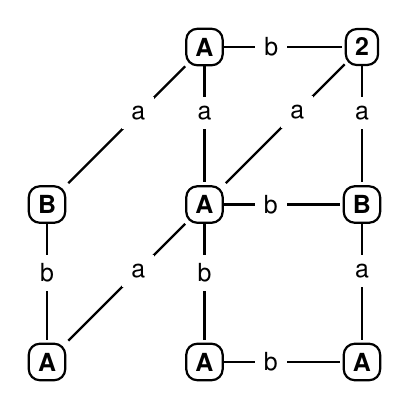
\begin{tikzpicture}[shorten >=1pt,auto,node distance=2cm,
                    thick,main node/.style={rounded corners,draw,font=\sffamily\small\bfseries}]

  \node[main node] (1) {A};
  \node[main node] (2) [right of=1] {2}; 
  \node[main node] (4) [below of =1] {A};
  \node[main node] (3) [left of=4] {B};
     \node[main node] (5) [below of=2] {B};
    \node[main node] (6) [below of=3] {A};
    \node[main node] (7) [below of=4] {A};
\node[main node] (8) [below of=5] {A};
  \path[every node/.style={font=\sffamily\small}]
    (1) edge[] node [minimum width = 1em, fill = white,pos=.25,right] {b} (2)
        edge[] node[minimum width = 1em, fill = white,pos=.25,below left] {a} (3)
        edge[] node[minimum width = 1em, fill = white,pos=.25,below] {a} (4)
    (2) edge[] node [minimum width = 1em, fill = white,pos=.25,below left] {a} (4)
        edge node [minimum width = 1em, fill = white,pos=.25,below] {a} (5)
    (3) edge[] node [minimum width = 1em, fill = white,pos=.25,below] {b} (6)
    (4) edge node [minimum width = 1em, fill = white,pos=.25,below] {b} (7)
    	edge[] node [minimum width = 1em, fill = white,pos=.25,below left] {a} (6) 
    	edge node [minimum width = 1em, fill = white,pos=.25,right] {b} (5) 
    (5) edge node [minimum width = 1em, fill = white,pos=.25,below] {a} (8)
    (7) edge node [minimum width = 1em, fill = white,pos=.25,right] {b} (8);	   
\end{tikzpicture}
\\\textbf{Step 3}
\end{minipage}
\begin{minipage}{.4\textwidth}
	\centering
	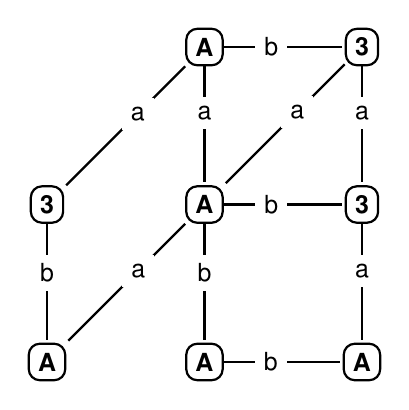
\begin{tikzpicture}[shorten >=1pt,auto,node distance=2cm,
                    thick,main node/.style={rounded corners,draw,font=\sffamily\small\bfseries}]

  \node[main node] (1) {A};
  \node[main node] (2) [right of=1] {3}; 
  \node[main node] (4) [below of =1] {A};
  \node[main node] (3) [left of=4] {3};
     \node[main node] (5) [below of=2] {3};
    \node[main node] (6) [below of=3] {A};
    \node[main node] (7) [below of=4] {A};
\node[main node] (8) [below of=5] {A};
  \path[every node/.style={font=\sffamily\small}]
    (1) edge[] node [minimum width = 1em, fill = white,pos=.25,right] {b} (2)
        edge[] node[minimum width = 1em, fill = white,pos=.25,below left] {a} (3)
        edge[] node[minimum width = 1em, fill = white,pos=.25,below] {a} (4)
    (2) edge[] node [minimum width = 1em, fill = white,pos=.25,below left] {a} (4)
        edge node [minimum width = 1em, fill = white,pos=.25,below] {a} (5)
    (3) edge[] node [minimum width = 1em, fill = white,pos=.25,below] {b} (6)
    (4) edge node [minimum width = 1em, fill = white,pos=.25,below] {b} (7)
    	edge[] node [minimum width = 1em, fill = white,pos=.25,below left] {a} (6) 
    	edge node [minimum width = 1em, fill = white,pos=.25,right] {b} (5) 
    (5) edge node [minimum width = 1em, fill = white,pos=.25,below] {a} (8)
    (7) edge node [minimum width = 1em, fill = white,pos=.25,right] {b} (8);	   
\end{tikzpicture}
\\\textbf{Step 4}
\end{minipage}\\
\hfill \vspace{5mm}\hfill \\
\begin{minipage}{.4\textwidth}
	\centering
	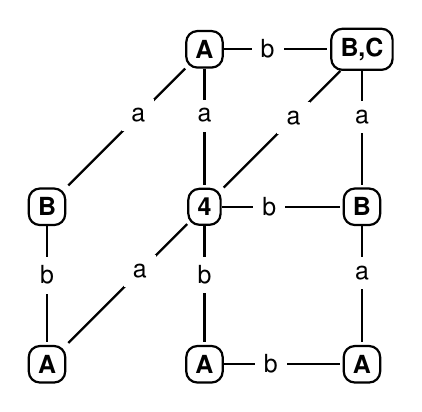
\begin{tikzpicture}[shorten >=1pt,auto,node distance=2cm,
                    thick,main node/.style={rounded corners,draw,font=\sffamily\small\bfseries}]

  \node[main node] (1) {A};
  \node[main node] (2) [right of=1] {B,C}; 
  \node[main node] (4) [below of =1] {4};
  \node[main node] (3) [left of=4] {B};
     \node[main node] (5) [below of=2] {B};
    \node[main node] (6) [below of=3] {A};
    \node[main node] (7) [below of=4] {A};
\node[main node] (8) [below of=5] {A};
  \path[every node/.style={font=\sffamily\small}]
    (1) edge[] node [minimum width = 1em, fill = white,pos=.25,right] {b} (2)
        edge[] node[minimum width = 1em, fill = white,pos=.25,below left] {a} (3)
        edge[] node[minimum width = 1em, fill = white,pos=.25,below] {a} (4)
    (2) edge[] node [minimum width = 1em, fill = white,pos=.25,below left] {a} (4)
        edge node [minimum width = 1em, fill = white,pos=.25,below] {a} (5)
    (3) edge[] node [minimum width = 1em, fill = white,pos=.25,below] {b} (6)
    (4) edge node [minimum width = 1em, fill = white,pos=.25,below] {b} (7)
    	edge[] node [minimum width = 1em, fill = white,pos=.25,below left] {a} (6) 
    	edge node [minimum width = 1em, fill = white,pos=.25,right] {b} (5) 
    (5) edge node [minimum width = 1em, fill = white,pos=.25,below] {a} (8)
    (7) edge node [minimum width = 1em, fill = white,pos=.25,right] {b} (8);	   
\end{tikzpicture}
\\\textbf{Step 5}
\end{minipage}
\begin{minipage}{.4\textwidth}
	\centering
	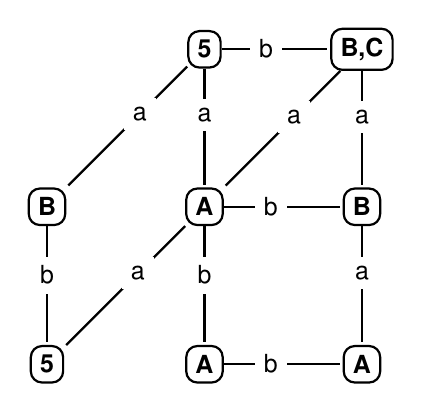
\begin{tikzpicture}[shorten >=1pt,auto,node distance=2cm,
                    thick,main node/.style={rounded corners,draw,font=\sffamily\small\bfseries}]

  \node[main node] (1) {5};
  \node[main node] (2) [right of=1] {B,C}; 
  \node[main node] (4) [below of =1] {A};
  \node[main node] (3) [left of=4] {B};
     \node[main node] (5) [below of=2] {B};
    \node[main node] (6) [below of=3] {5};
    \node[main node] (7) [below of=4] {A};
\node[main node] (8) [below of=5] {A};
  \path[every node/.style={font=\sffamily\small}]
    (1) edge[] node [minimum width = 1em, fill = white,pos=.25,right] {b} (2)
        edge[] node[minimum width = 1em, fill = white,pos=.25,below left] {a} (3)
        edge[] node[minimum width = 1em, fill = white,pos=.25,below] {a} (4)
    (2) edge[] node [minimum width = 1em, fill = white,pos=.25,below left] {a} (4)
        edge node [minimum width = 1em, fill = white,pos=.25,below] {a} (5)
    (3) edge[] node [minimum width = 1em, fill = white,pos=.25,below] {b} (6)
    (4) edge node [minimum width = 1em, fill = white,pos=.25,below] {b} (7)
    	edge[] node [minimum width = 1em, fill = white,pos=.25,below left] {a} (6) 
    	edge node [minimum width = 1em, fill = white,pos=.25,right] {b} (5) 
    (5) edge node [minimum width = 1em, fill = white,pos=.25,below] {a} (8)
    (7) edge node [minimum width = 1em, fill = white,pos=.25,right] {b} (8);	   
\end{tikzpicture}
\\\textbf{Step 6}
\end{minipage}
\caption{Algorithm Data Graph Processing}
 \label{fig:workingdg}
\end{figure}
\par In the data graph, the singleton NEC's are given according to the label of the node. In step 2 and Step 3 the nodes are getting NEC 1 and NEC 2 because the nodes matches the node label. NEC 1 and NEC 2 has no children to check. In step 4 the nodes are getting NEC 3 if it has a child with NEC 1 by an edge label 'a'. Then in step 5 the nodes are getting NEC 4 if it has a child of NEC 2 by edge label 'a'. In the final step the NEC 5 is given for nodes with two children. Each step describes the candidate set for each of the NEC's. $CVS(NEC 1)$ has 5 nodes. $CVS(NEC 2)$ has 1 node. $CVS(NEC 3)$ has 3 nodes. Then a actual tree matching is done using these CVS. All the combination of CVS are tested to find all possibilities of matching the tree in data graph. After that the non tree edges are checked.
\section{Inferences}
\hspace{10mm}The parallel version needs to store the mapped NEC for each node in the data graph. This is asking for a space of $O(n*N(q))$ where $n$ is number of nodes in data graph and $N(q)$ is number of  NEC in query graph. The time taken for executing complete graphs on various test scenarios are given below. These results are obtained on a NVIDIA CUDA supported GPU with 580 MHz speed. Stage 1 is the NEC finding on Query Graph. Stage 2 is the CVS finding. Stage 3 is the matching.$100n1000e$ means 100 nodes and 1000 edges. 

\begin{figure}[h]
 \centering
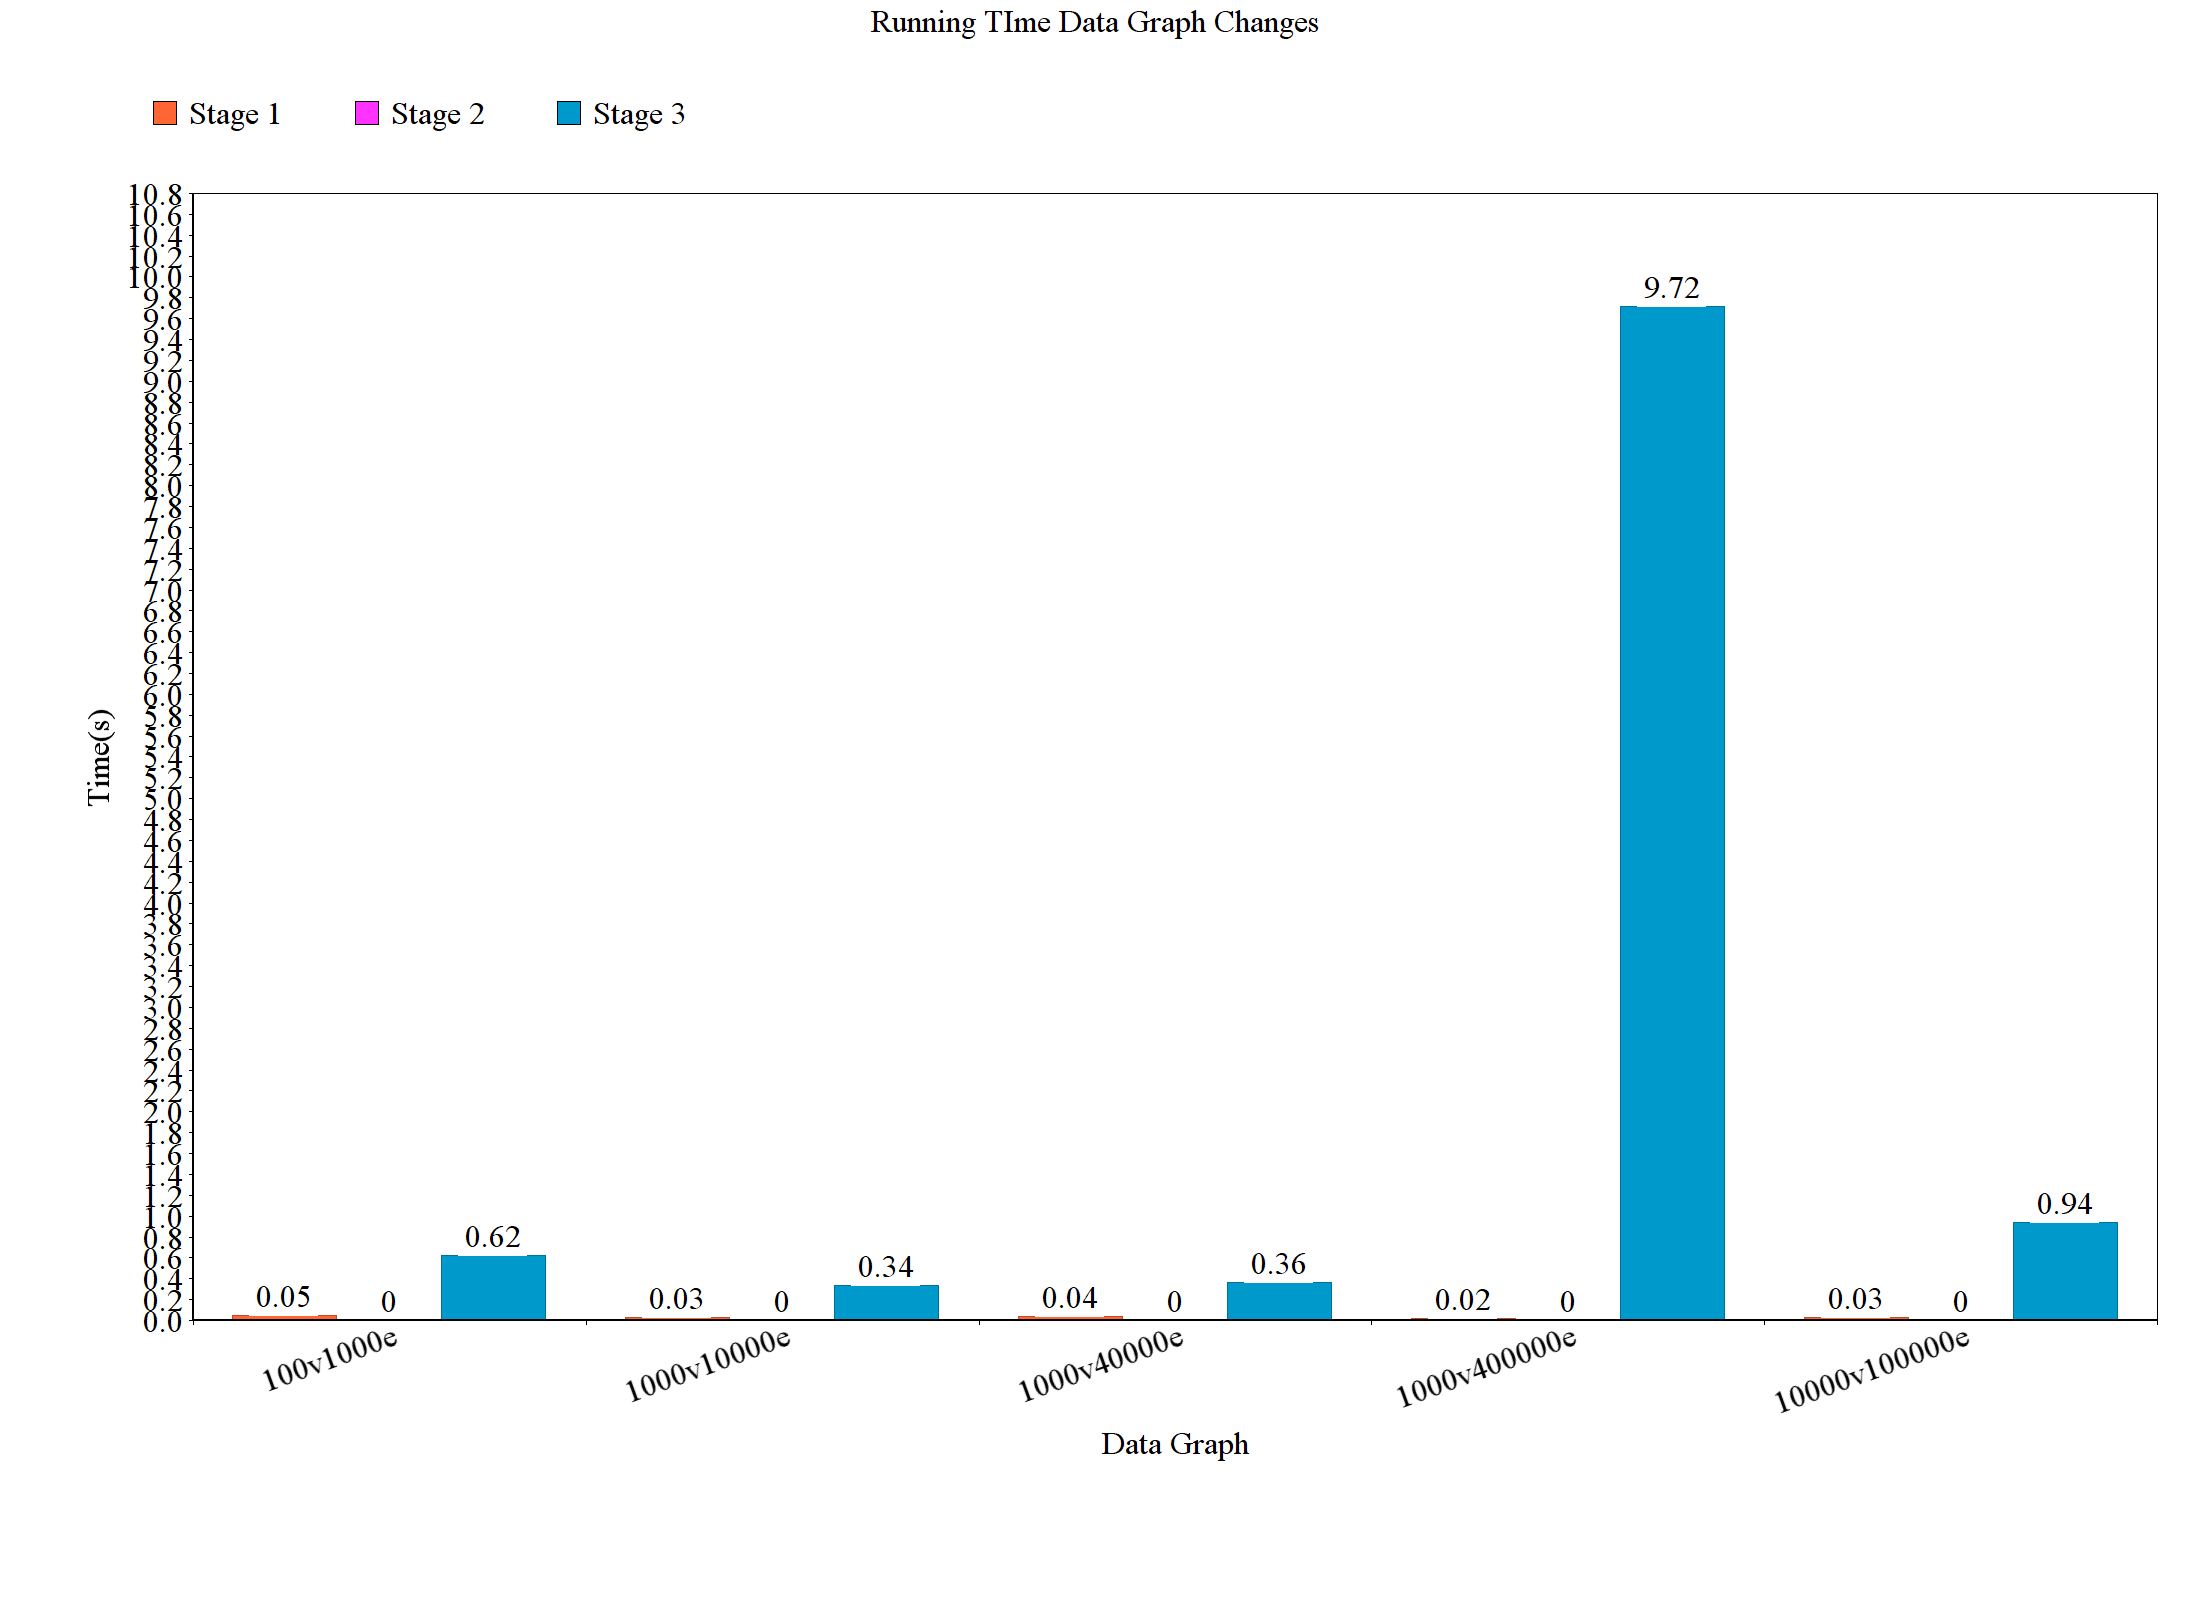
\includegraphics[width=.5\textwidth]{Dchange.png}
 \caption{Data Graph Size Changes}
 \label{fig:dchange}
\end{figure}
\hspace{10mm} When the data graph size changes the running times increases rapidly. The running time is depending on the density of the graph. If the size of the data graph increases and the density remains same, the running time doesn't show a spike. Fourth group shows a spike because of the huge density change from the other graphs. When the density changes the number of successful matching also increases causing the Stage 3(matching) to run more. \\
\begin{figure}[h!]
 \centering
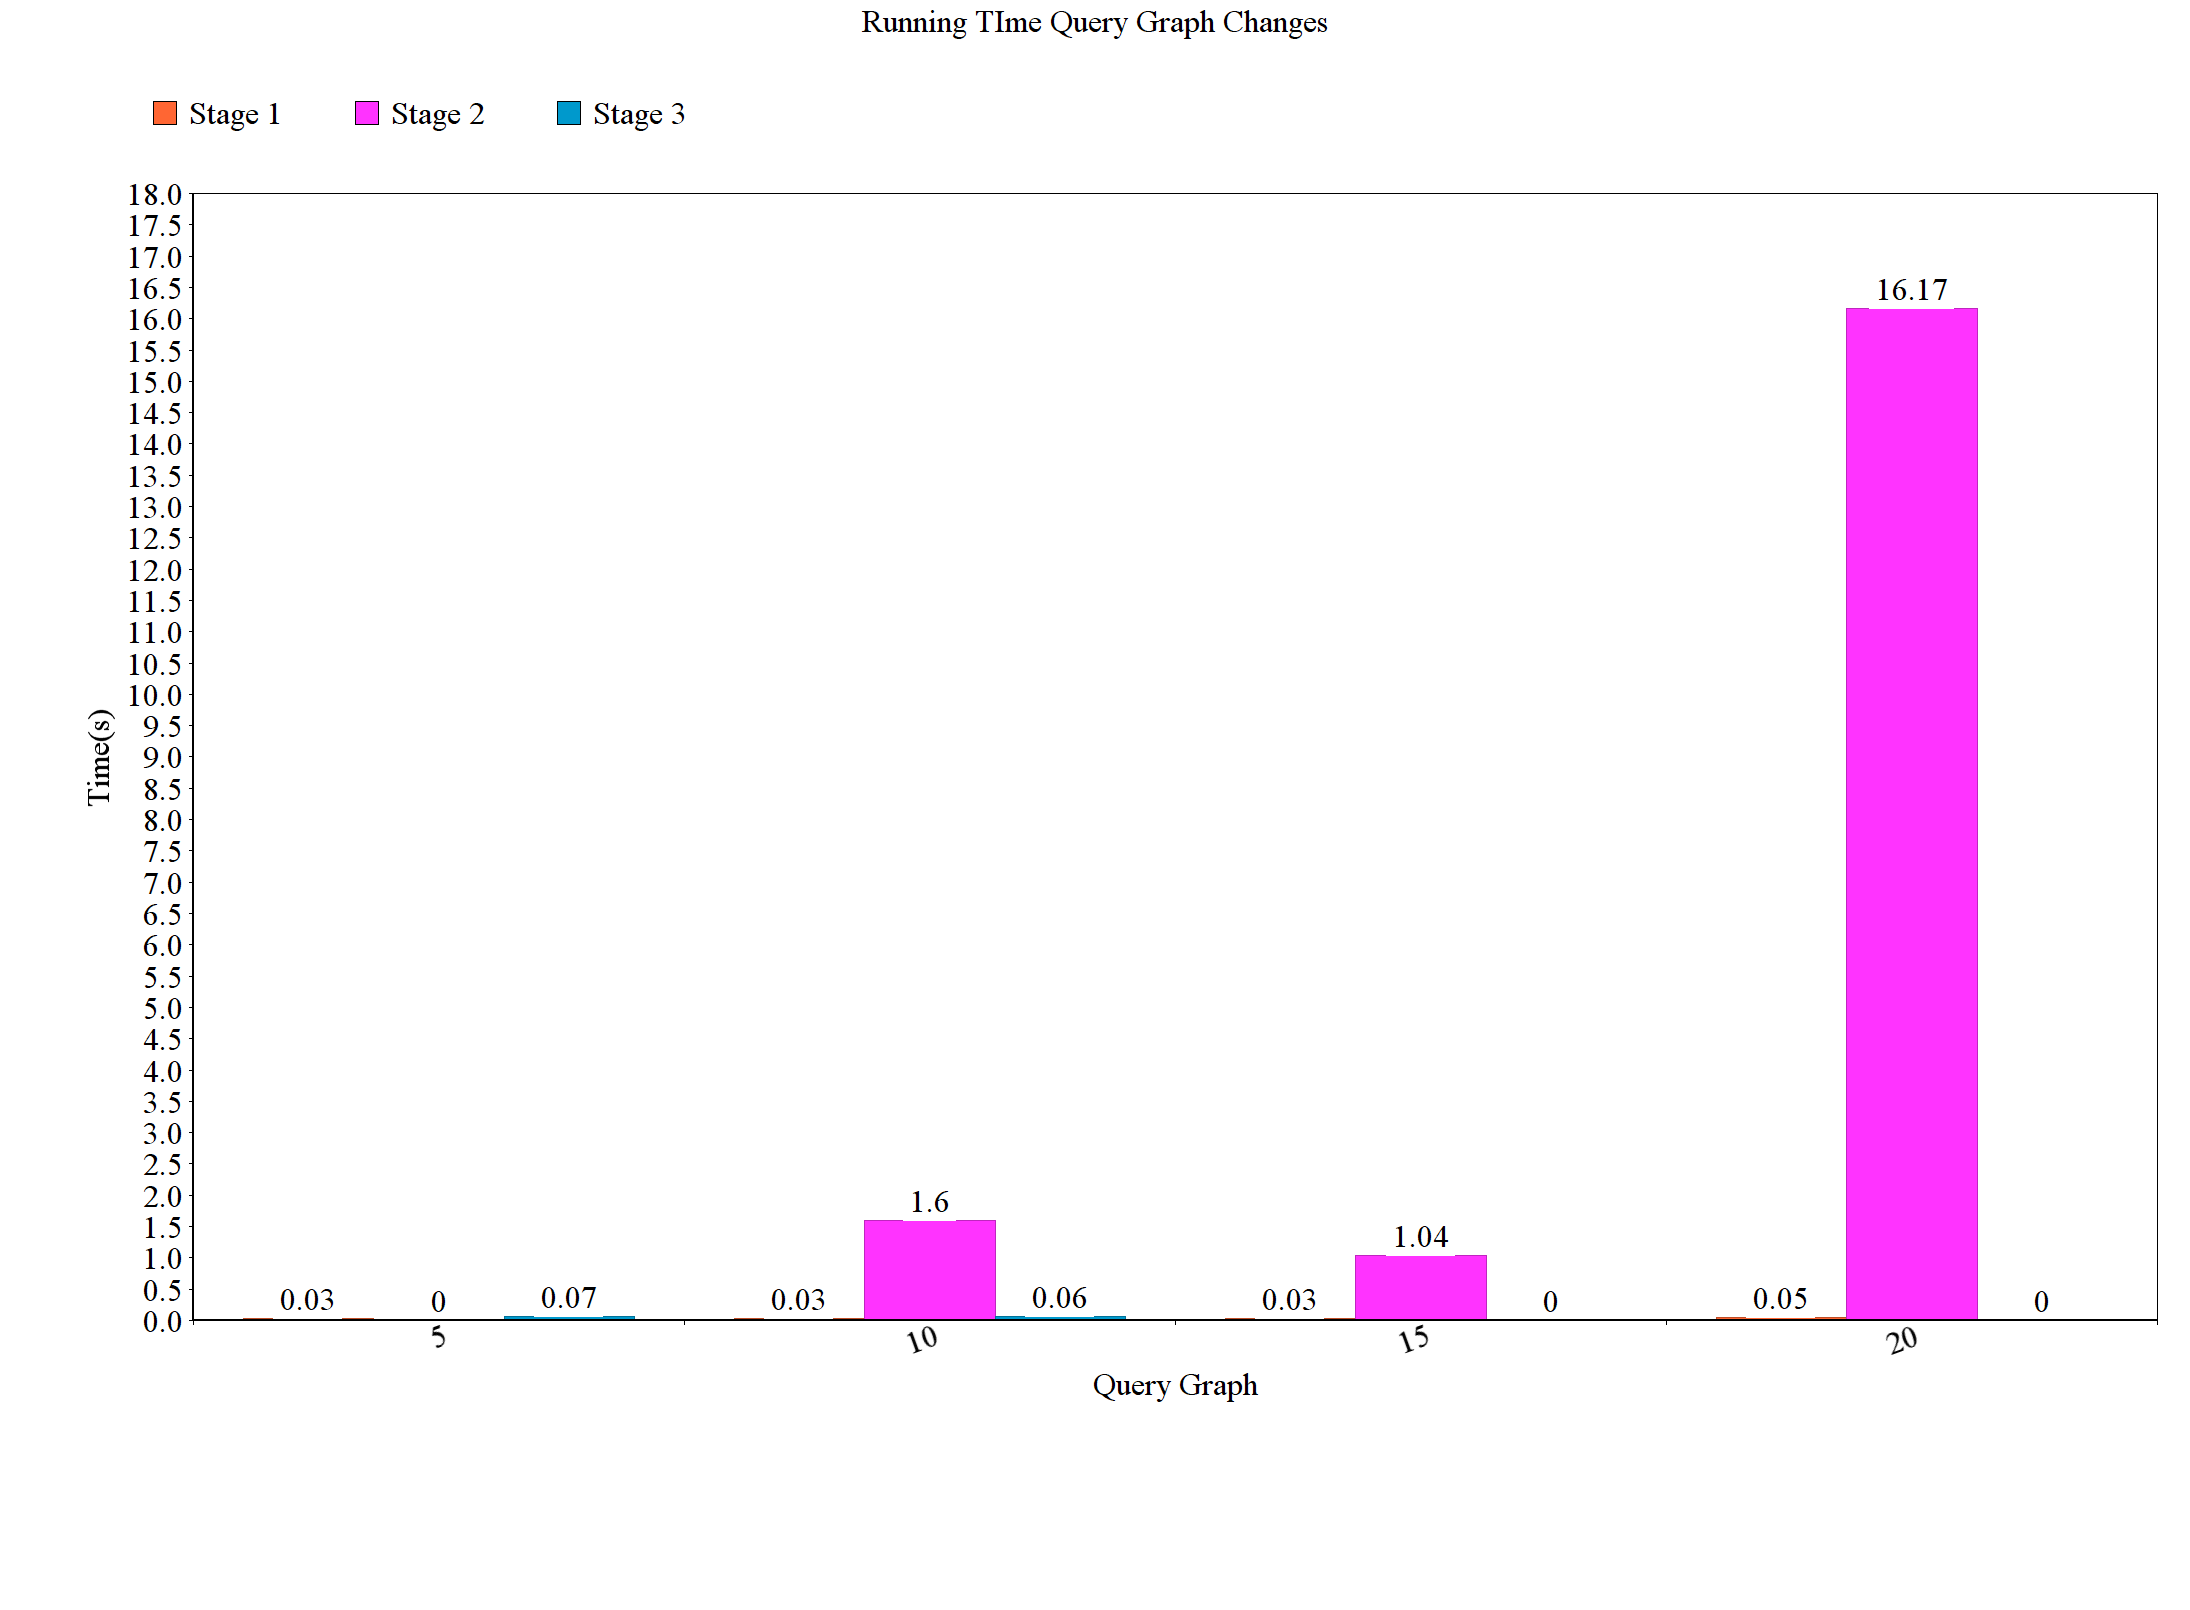
\includegraphics[width=.5\textwidth]{Qchange.png}
 \caption{Query Graph Size Changes}
 \label{fig:qchange}
\end{figure}
\hspace{10mm} When the query graph size changes the overall time increases. But the processing in Stage 2 is increased. The Stage 2 depends on the number of NEC. The NEC count will increase if the number of nodes in query graph increases. The Stage 3 is getting zero because the CVS becomes null set. No candidate would have been found for higher level nodes. This will help to not run Stage 3 making the time zero.\\
\begin{figure}[h!]
 \centering
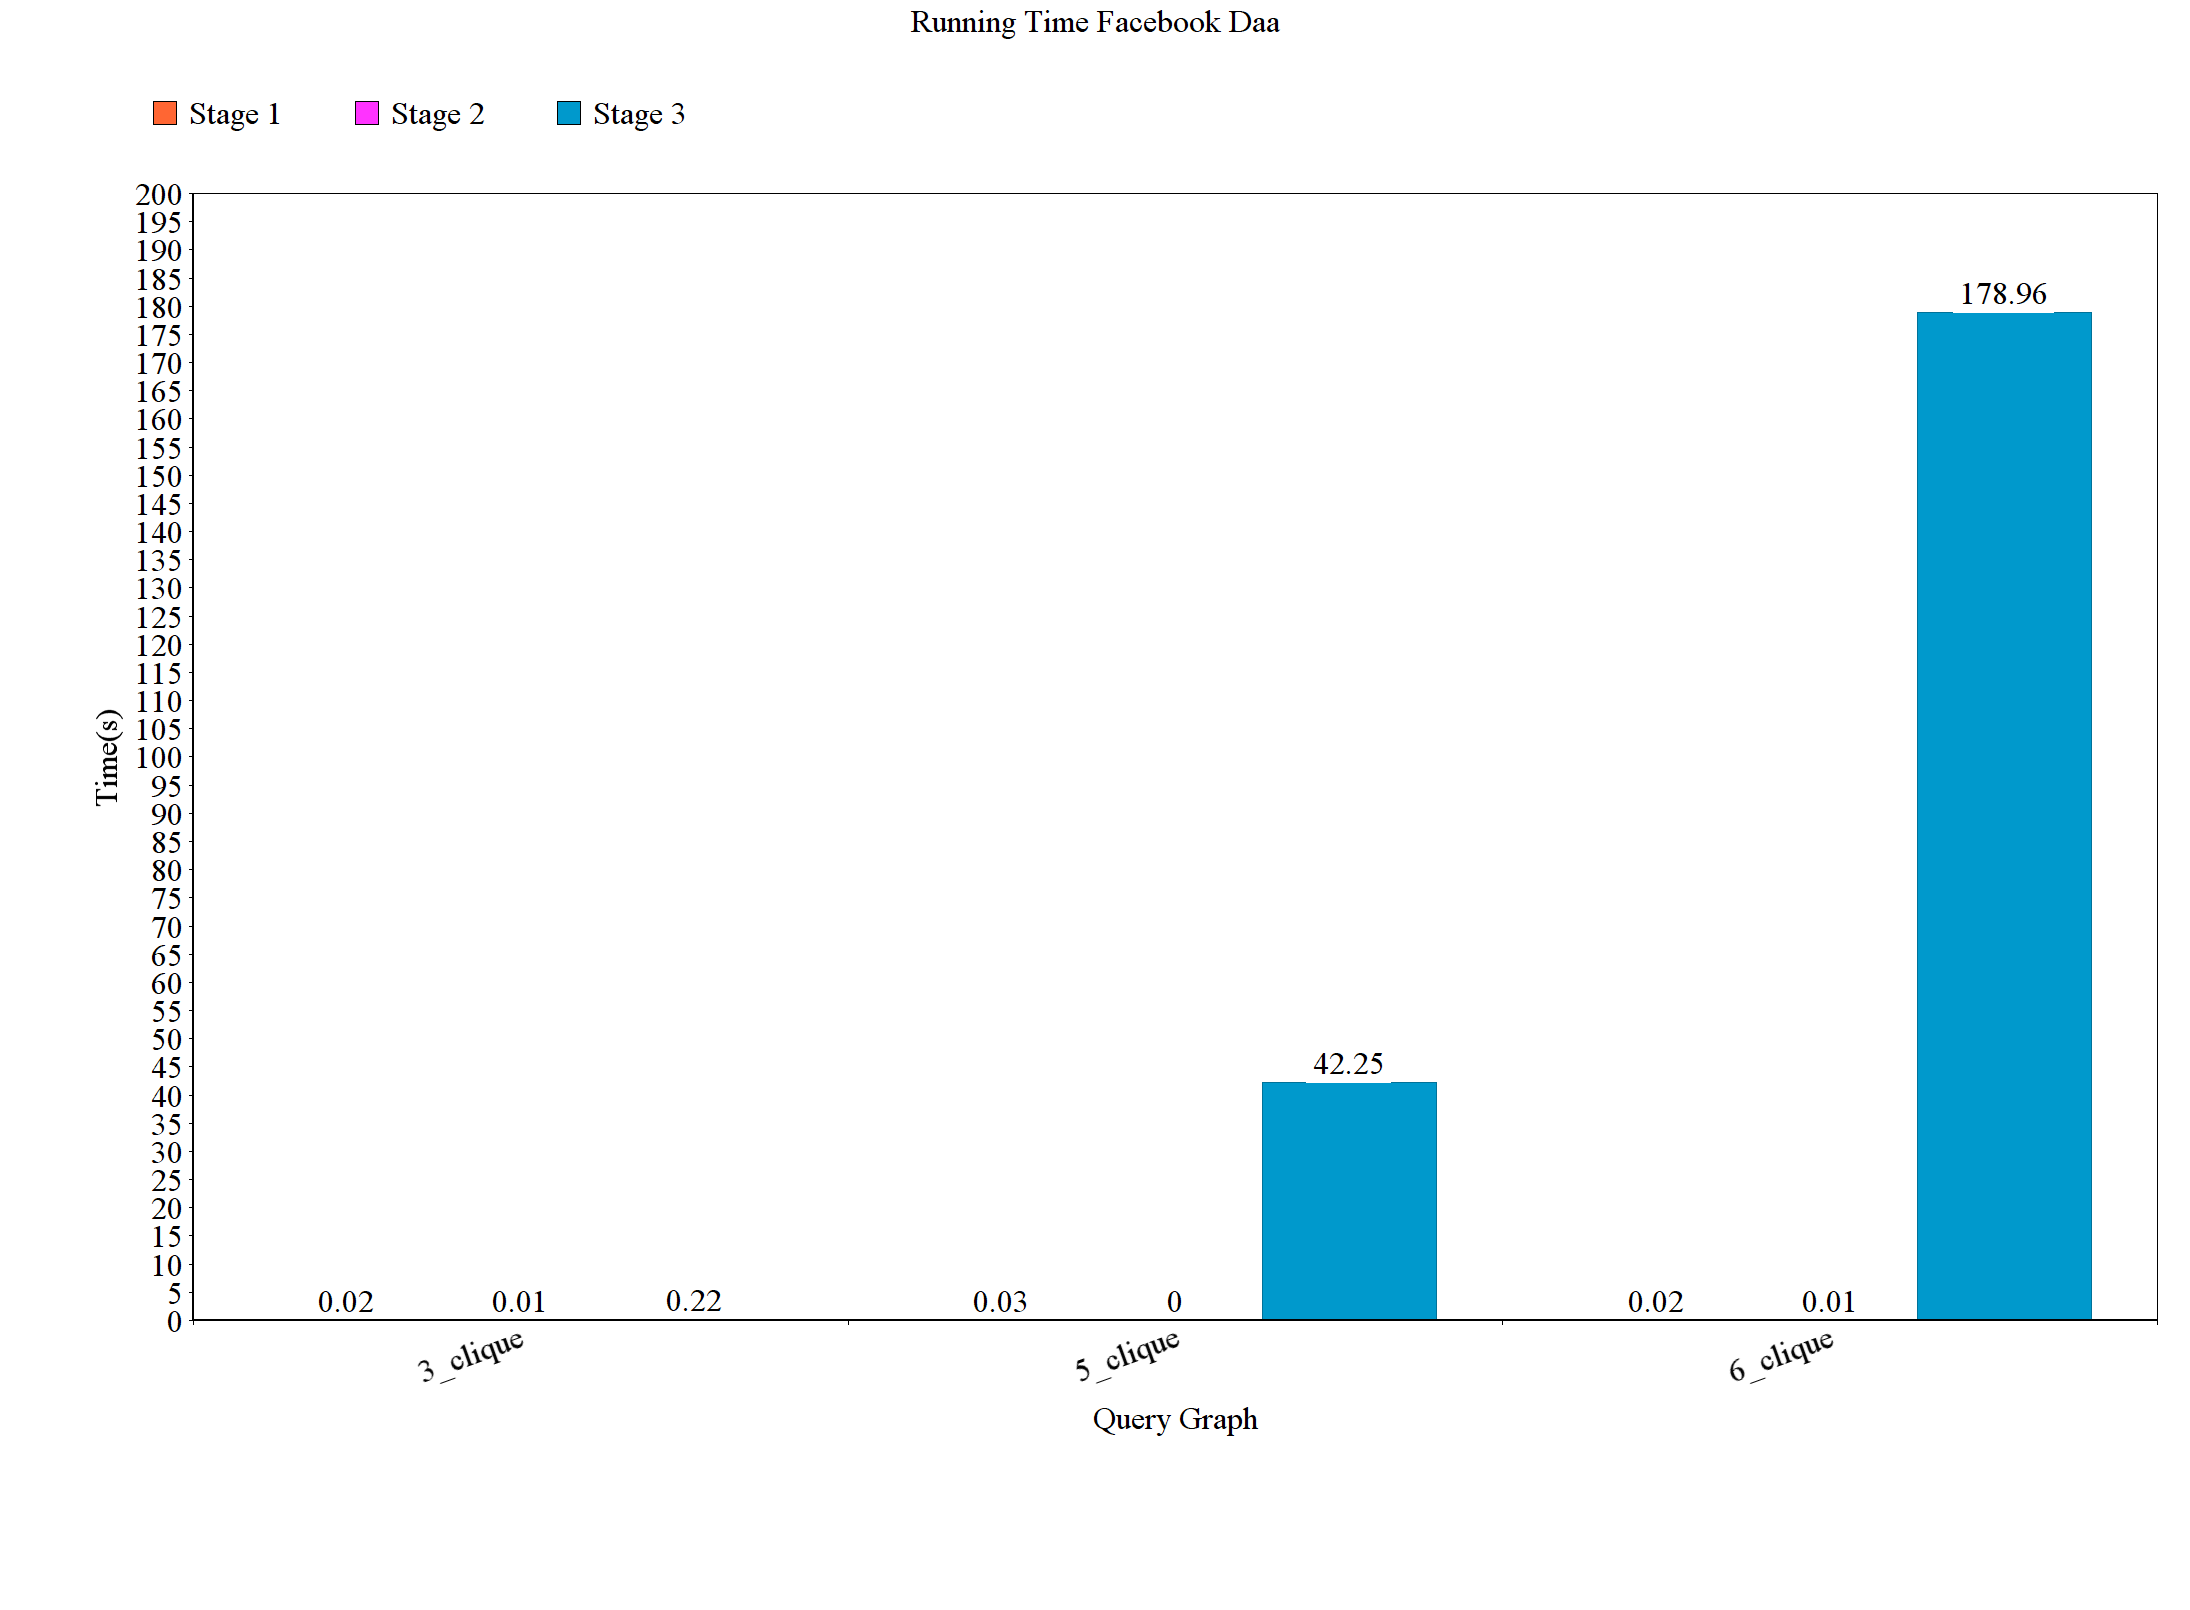
\includegraphics[width=.5\textwidth]{fb.png}
 \caption{Facebook network}
 \label{fig:fb}
\end{figure}
\hspace{10mm} Facebook Data is having 4039 nodes and 88234 edges making it a slightly dense network. Even if the final number of cliques of size 5 and 6 are in the range of number of triangle. Number of possible checks requires increases. Each node addition will cause to calculate almost 100(from CVS size) more possibilities. The false candidates are not easy to remove since the graph is fairly dense.\\
\begin{figure}[h!]
 \centering
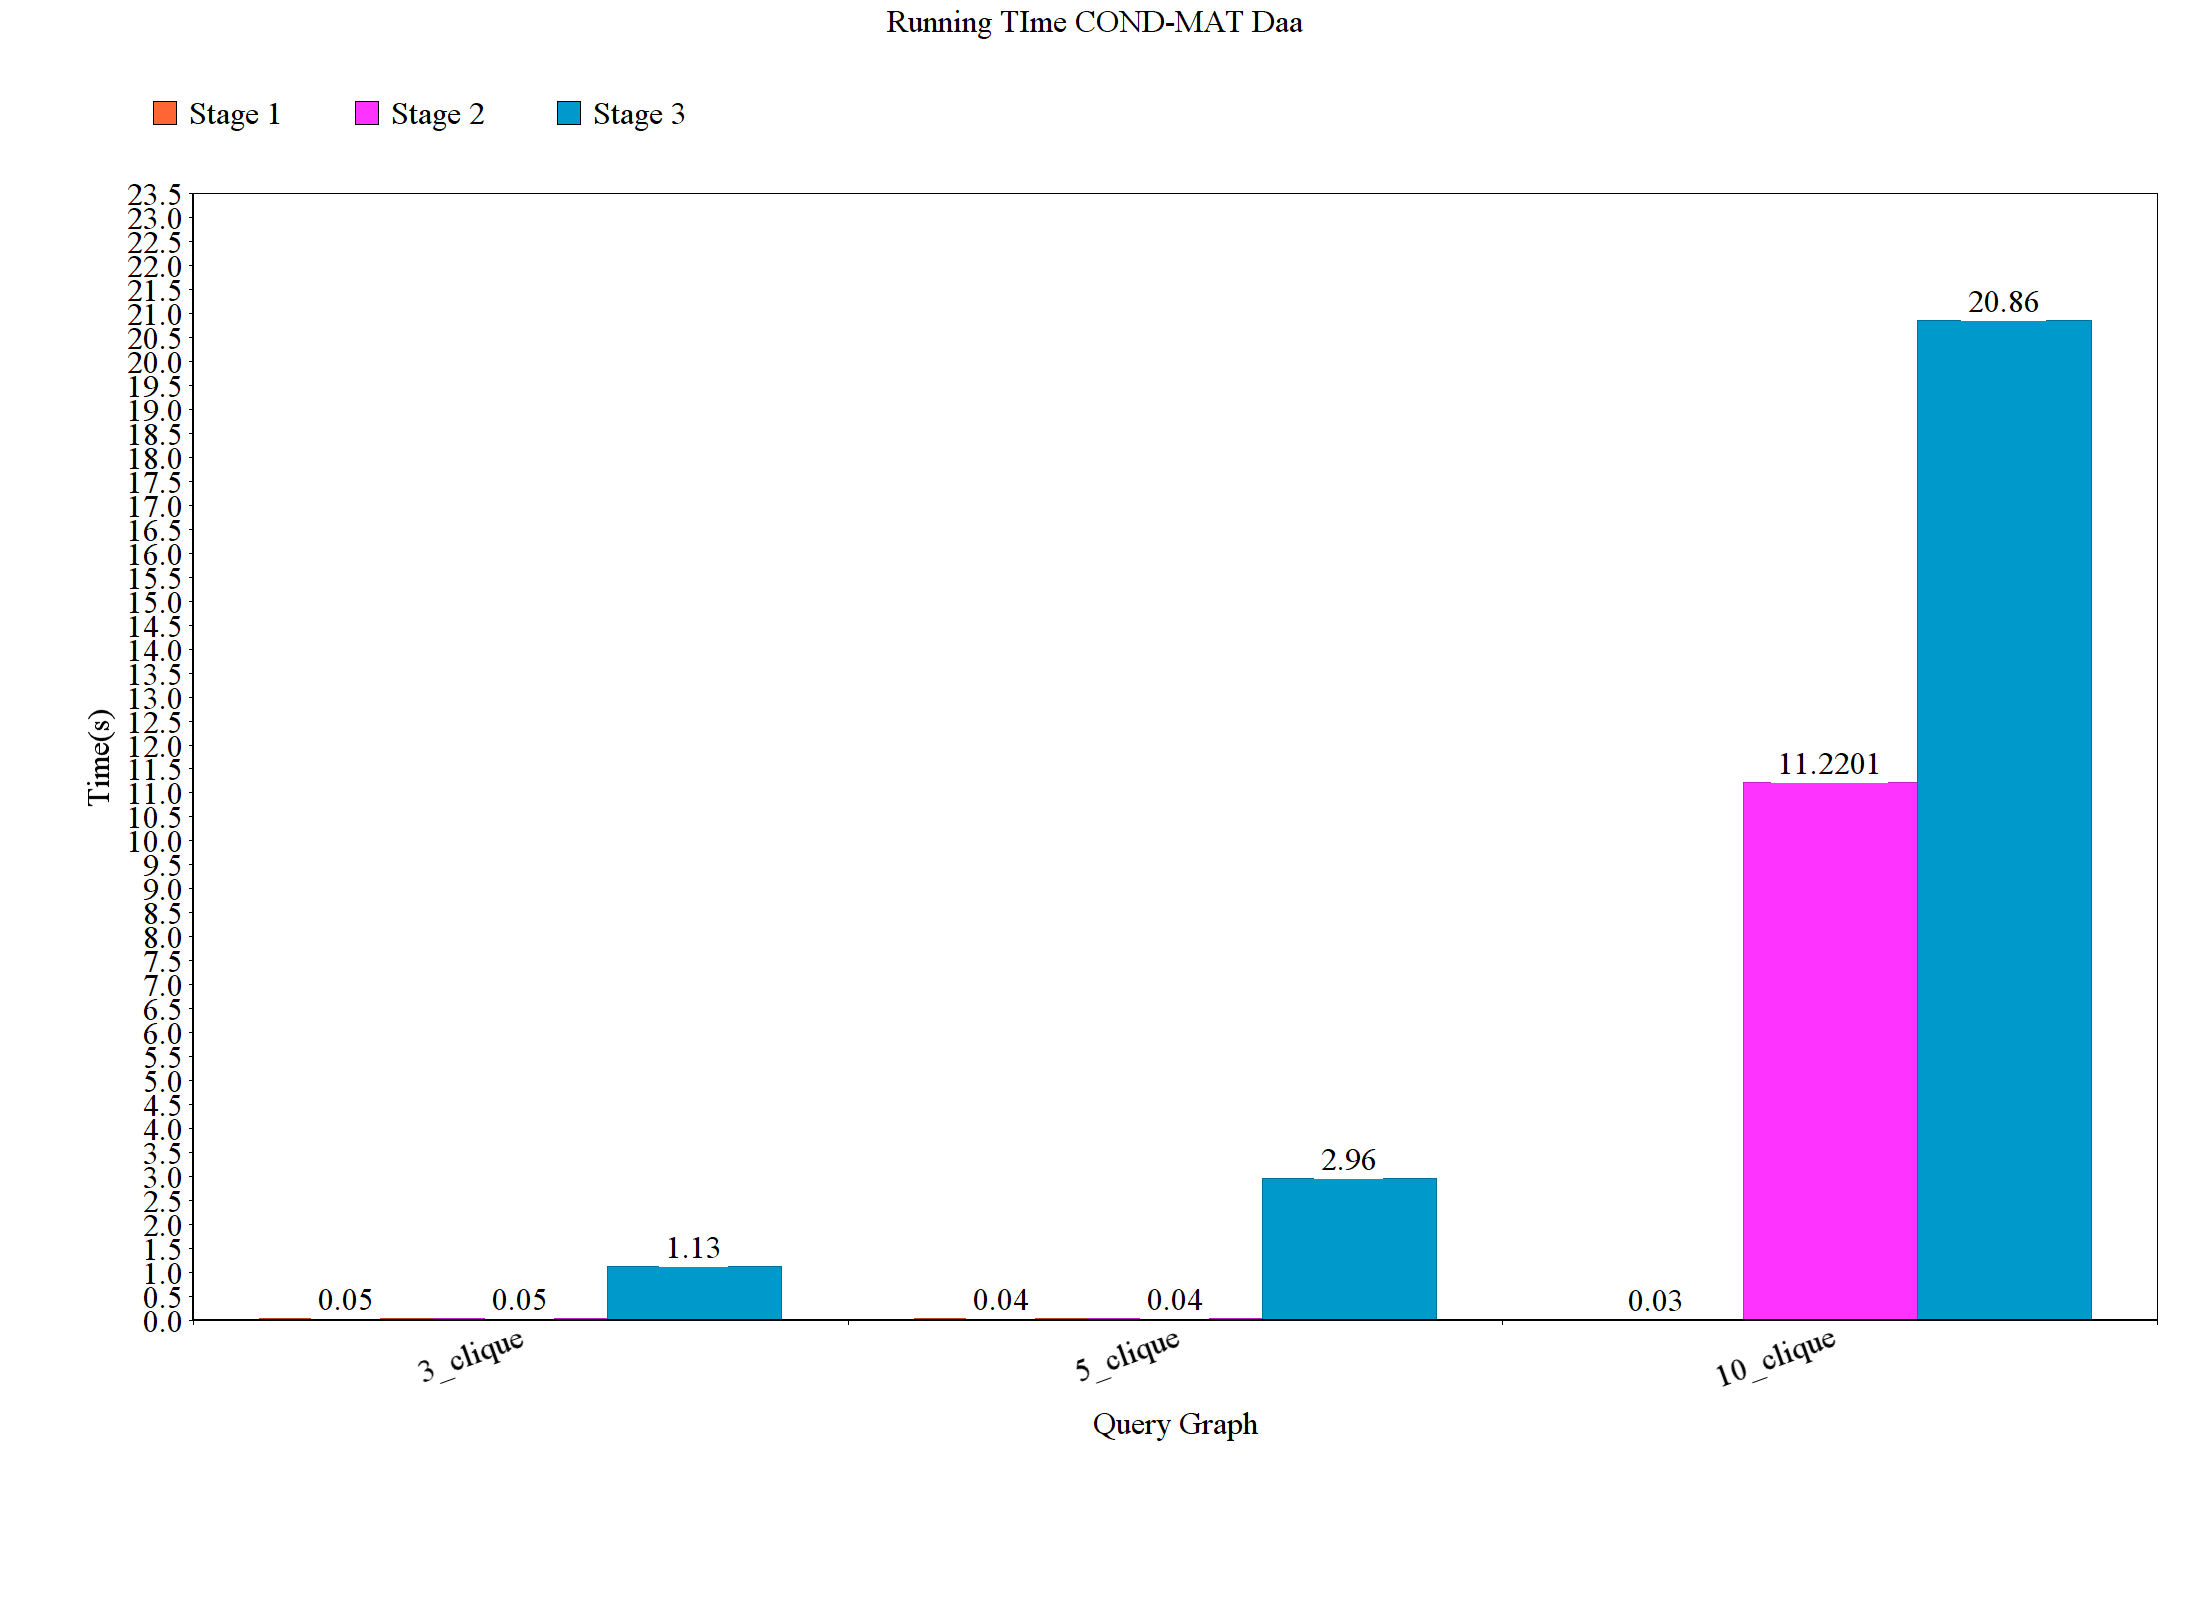
\includegraphics[width=.5\textwidth]{CA.png}
 \caption{Condense Matter collaboration network}
 \label{fig:ca}
\end{figure}
\hspace{10mm}Condense Matter collaboration network Dataset is having 23133 nodes and 93497 edges. The graph is slightly sparse. The number of higher node cliques are less and the possibilities of finding them is also getting reduced due to the sparsity of the graph. The increase in time is not that steep because of the low density.
\section{Failed Approach}
	\hspace{10mm}We tried to make the the NEC numbering more informative by using primes and composites. A prime will be assigned to a class if that graph has no other embedding of any previous graphs we came across. If it has the embedding we give product of the prime numbers of the embedding. This method helps to know that if the NEC has a composite number it has some smaller graphs embedded in it. So we won't be needed to  search the sub-graphs in this node.\\
\hspace{10mm}	It actually captures all sub-graphs at the root. See the figure \ref{fig:NEC}.\\
	\begin{figure}[h]
 \centering
%\centering
\begin{minipage}{.6\textwidth}
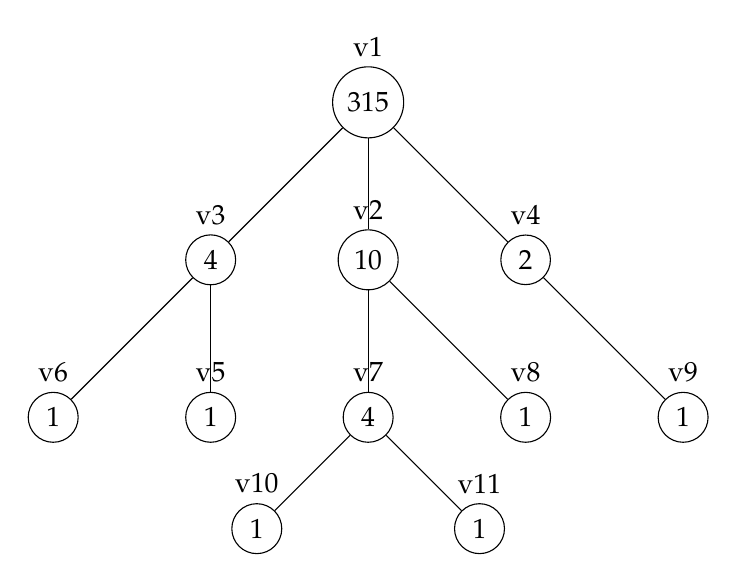
\begin{tikzpicture}[node distance=2cm]
\node[circle,draw,label=v1] (1)[]{315};
\node[circle,draw,label=v2] (3)[below of=1]{10};
\node[circle,draw,label=v3] (2)[left of=3]{4};
\node[circle,draw,label=v4] (4)[ right of=3]{2};
\node[circle,draw,label=v5] (5)[below of=2]{1};
\node[circle,draw,label=v6] (6)[left of=5]{1};
\node[circle,draw,label=v7] (7)[below of=3]{4};
\node[circle,draw,label=v8] (8)[right of=7]{1};
\node[circle,draw,label=v9] (9)[right of=8]{1};
\node[circle,draw,label=v10] (10)[below left of=7]{1};
\node[circle,draw,label=v11] (11)[below right of=7]{1};
\path
	(1) edge node{} (2)
		 edge node{} (3)
		 edge node{} (4)
	(2) edge node{} (5)
		edge node{} (6)
	(3) edge node{} (7)
		edge node{} (8)
	(4) edge node{} (9)
	(7) edge node{} (10)
		edge node{} (11);	
\end{tikzpicture}
\end{minipage}
\begin{minipage}{.2\textwidth}
\centering
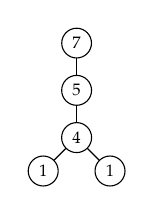
\begin{tikzpicture}[scale=0.1,every node/.style={scale=0.6}]
\node[circle,draw] (5)[]{7};
\node[circle,draw] (1)[below of=5]{5};
\node[circle,draw] (2)[below of=1]{4};
\node[circle,draw] (3)[below left of=2]{1};
\node[circle,draw] (4)[below right of=2]{1};
\path
	(5) edge node{} (1)
	(1) edge node{} (2)
	(2)	 edge node{} (3)
		 edge node{} (4);
\end{tikzpicture}\\Intermediate graph \hfill \\
\begin{tikzpicture}[scale=0.1,every node/.style={scale=0.6}]

\node[circle,draw] (1)[]{3};
\node[circle,draw] (2)[below of=1]{2};
\node[circle,draw] (3)[below of=2]{1};
\path
	(5) edge node{} (1)
	(1) edge node{} (2)
	(2)	 edge node{} (3);
\end{tikzpicture}
\\Intermediate Graph
\end{minipage}
 \caption{NEC based on primes}
 \label{fig:NEC}
\end{figure}
\hspace{10mm}  $v4$ is getting 2 since it has only one child $1$. $v7$ and $v3$ gets 4 since it has two same sub-graphs(sub-graph $2$) inside them. $v2$ is getting 10 since it has sub-graph $2$ and $5$ (see the numbering shown on right). Similarly $v1$ has two $3$s($v2$ contributes one $3$) ,one $7$ and one $5$.

 \hspace{10mm}	But this was not effective.When we consider the data graph we will need to store only one integer the product of all the graphs inside that node. The first problem we faced was the value of composite number can go beyond the long integer limit. So we tried only storing primes. But that also didn't make much difference. By our propagation algorithm in Data Graph, we start by giving id $1$ to all nodes in the data graph in the first iteration. In the second iteration every node will get id $2$ since every node will have a child of id $1$. Then in third every node will get $3$ and so on. So every node gets every id present in query graph.
 
 \hspace{10mm} It only helped as in knowing whether there exist a path of length matching the largest length path in query graph. This will lead to all nodes becoming a candidate for the final search we atleast one graph existed in the connected component. So it is not making the CVS tight.
	
\chapter{Dynamic Operations}
 \label{chap:dynamic}
 \section{Introduction}
	\hspace{10mm} The dynamic operations are add/delete operation on either query or data graph. The dynamic version is also having large applications. The dynamic processing will help to generate the isomorphic mappings without computing the whole answer again. This will give a great improvement in time. The dynamic changes are allowed with one condition that the query or graph will remain connected at any point of time. The dynamic queries are processed non-deterministic-ally meaning the order of execution of the dynamic queries is undefined. 
	\hspace{10mm} The dynamic operations and its difficulties are shown below.
	\begin{table}[H]
\centering
\begin{tabular}{|m{4cm}|m{4cm}|m{4cm}|m{4cm}|}
\hline
\textbf{}                                  & \textbf{Query Add Edge}                     & \textbf{Query Remove edge}                                 & \textbf{Query Unchanged} \\ \hline
\textbf{Data Add Edge}                                  & \textbf{Easy}                     & \textbf{Difficult}                                 & \textbf{Easy} \\ \hline
\textbf{Data Remove Edge}                                  & \textbf{Easy}                     & \textbf{Difficult}                                 & \textbf{Easy} \\ \hline
\textbf{Data Unchanged}                                  & \textbf{Easy}                     & \textbf{Difficult}                                 & \textbf{Static} \\ \hline
\end{tabular}
\caption{Dynamic Changes Difficulty Level}
%\label{tab:lit}
\end{table}
\section{Intermediate Answers}
	The intermediate answers will be saved so that dynamic answers can be processed faster.
	\begin{figure}[h]
 \centering
%\centering
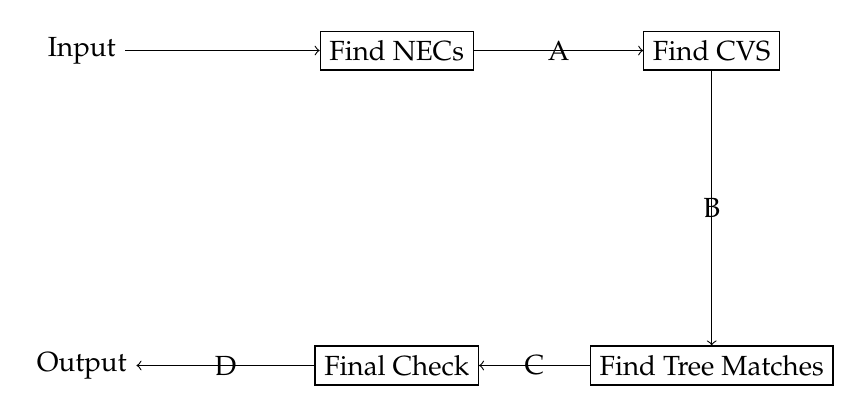
\begin{tikzpicture}[node distance=4cm]
\node[draw=none](6)[]{Input};
\node[rectangle,draw] (1)[right of=6]{Find NECs};
\node[rectangle,draw] (2)[right of=1]{Find CVS};
\node[rectangle,draw] (3)[below of=2]{Find Tree Matches};
\node[rectangle,draw] (4)[left of=3]{Final Check};
\node[draw=none](5)[left of =4]{Output};
\path[->]
	(6) edge node{} (1)
	(1) edge node{A} (2)
	(2) edge node{B} (3)
	(3) edge node{C} (4)
	(4) edge node {D} (5);
\end{tikzpicture}

 \caption{Intermediate Answers}
\end{figure}
	\hspace{10mm} A,B,C,D are the intermediate answer saved variables. A store the NECs of each vertec in query graph. B store CVS of each query vertex in data graph. C store the possible tree matches. D store the final exact graph maps.
\section{Adding Edge to Query Graph}
 \label{sec:aq}
	\hspace{10mm} It one of the easiest case because we need to check all the previous cases. The final answer will be a subset of previous answer.ie; Some of the matching will become invalid since the added edge may not be present. Only D changes.
	\hspace{10mm} Multiple queries can be done in parallel  by checking the existence of the added edges in all the previous answers. In parallel on all previous answers check the presence of added edges.
\section{Deleting Edge from Data Graph}
 \label{sec:dd}
	\hspace{10mm} It is also easy because the final answer is subset of previous answer.Multiple Queries can be processed similiar to the previous case.Only D changes.
	\hspace{10mm} Even if we needed to 
\section{Deleting Edge from Query Graph}
 \label{sec:dq}
	\hspace{10mm} This is a difficult case since we need to find the mappings that are going to be added. This case is divided into two parts.
\subsection{Deleting a non-tree edge}	
	\hspace{10mm} The tree inside the query graph remains unchanged. So the tree matches are correct. We need to go through all the tree matching(C) and check for possible additions of maps to final answer. So saving the intermediate answer C helps in finding the solution faster.
\subsection{Deleting a tree edge}	
	\hspace{10mm} Since the tree is changed here the CVS of vertices may change.So rather than calculating all the CVS there is a more efficient way. If a edge u-v in the tree is deleted and u is parent of v in tree. All the nodes in the path from u to root(parent,grand-parent,.. of u) should recalculate the CVS.
	 \hspace{10mm} When multiple queries are given the deletion may be from different parts of the tree. But each node should be processed once. 
\begin{algorithm}[H]
\caption{Dynamic tree edge deletion of thread t}
\textbf{Input}: Data Graph $D$,Query Graph $Q$,Delete u-v(u is parent of v).\\
\textbf{Output}: CVS updates.\\
\begin{algorithmic}
 \item \begin{enumerate}
 \item w=v
\item for each parent of w(till root)
 \begin{enumerate}
\item mark w for t
\end{enumerate}
\item for each parent of w(till root)
 \begin{enumerate}
\item if mark at w is t, acquire lock for w
\end{enumerate}
\item for each parent of w(till root)
\begin{enumerate}
\item if mark at w is t and able to acquire locks for all childs of w 
\item Recompute NEC of w
\item if not a previously computed NEC then
\item  \hspace{10mm}C(w)=$FindCandidates$(w,D) update
\item Release all locks
\end{enumerate}
\end{enumerate}
\end{algorithmic}
\end{algorithm}
	\hspace{10mm} The above algorithm marks all the parent nodes from a particular deleted edge. This marking helps to make sure only one thread process one node. The processing will be done such a way that no parent nodes are processed if any  child of the parent is unprocessed. So the processing order will be leaf to root. This will change the values inside A and so as B.
\section{Adding Edge in Data Graph}
 \label{sec:ad}
	\hspace{10mm} This will also add entries into B. But A will not be changed since no edges in query graph is changed. 
	\begin{algorithm}[H]
\caption{Dynamic data edge addition of thread t}
\textbf{Input}: Data Graph $D$,Query Graph $Q$,Delete u-v(u is parent of v).\\
\textbf{Output}: CVS updates.\\
\begin{algorithmic}
 \item \begin{enumerate}
 \item w=v (for u also)
\item for each child of w(till $|Q|$ length)
\begin{enumerate}
\item if acquire locks for all childs of w 
\item foreach NEC's x
\item C(x)=$FindCandidates$(x,D) update
\item Release all locks
\end{enumerate}
\end{enumerate}
\end{algorithmic}
\end{algorithm}
\hspace{10mm} This algorithm moves to  $|Q|$ length from both u and v in a BFS fashion. At each Data node it is checked whether it can be added to CVS of any of the NECs. When there is an overlap of regions of different thread locks are used to synchronize them. Since the Data graph is huge and  query graph is small and so the possibility of two edge deletion happening near( edge length  $< ~|Q|$ ) is small, the number of locks waits will be minimal.
\subsection{Parallel Execution}
\hspace{10mm} All the four quires can be processed in parallel since they are operating on different data. \ref{sec:aq} and \ref{sec:dd} are processing on D while \ref{sec:dq} and \ref{sec:ad} are processing on A and B. So it is safe to run them parallel. Parallel adding to A and B doesn't make the answer inconsistent. It will add a vertex into the CVS which  will be removed when exact matching is performed in the end.
\subsection{Inferences}
	\hspace{10mm} So a $Find Tree$ match algorithm should be done at each stage of the output to get the new possiblities. But this stage is the costliest of all the four steps. Even one vertex is added to any two CVS, this will cause to recompute most of the permutations and combinations again. So there is no computational advantage by dynamic processing. Running a subgraph isomorphism solution after applying all edge updates becomes equally fast as the dynamic version. 

%\include{parts/chapters/experiments}                                                                                
\chapter{CONCLUSION AND FUTURE WORK}
\label{chap:concl}

\section{Conclusion}

\hspace{10mm} The state-of-art algorithms for Subgraph Isomorphism use different pruning techniques to avoid the false candidates as early as possible.  The part of the algorithm which considers all possibility is the most time consuming part. Since we can't avoid checking some possibility the one efficient way of making this part faster is decreasing the number of candidates. The complexity of the pruning technique helps to remove more false candidates thus  making the algorithm faster. The possibility checking part is made faster by using GPU by checking different possibilities in different threads. Thus a million possibilities are checked in parallel.\\
\hspace{10mm} The dynamic version of the problem is trying to answer the problem after many edge deletions and additions. The trivial cases are the adding in query and deletion in data. The other two cases makes the problem hard. Whether there exists a faster method(poly-time) for processing them in parallel still remains as an open problem. 




%%%%%%%%%%%%%%%%%%%%%%%%%%%%%%%%%%%%%%%%%%%%%%%%%%%%%%%%%%%%
% Appendices.
%\appendix
\label{app:class}
\chapter{CLASSIFICATION AND FEATURE EXTRACTION TECHNIQUES USED}
\section{Classification Techniques}
\subsection{Gaussian Mixture Model}
In statistics, a mixture model is a probabilistic model for representing the presence of subpopulations within an overall population. As the name indicates, train data is modeled as a mixture of Gaussian functions. This is basically linear superposition of Gaussians in the form\\
 \begin{equation}
 p(x) = \sum_{k=1}^{K}\pi_{k}N(x|\mu_{k},\Sigma_{k})
 \end{equation}
The biggest advantage of clustering using Gaussian mixture model over traditional clustering method is that each point can be represented more than one cluster. So, it is kind of best way to represent multi modality in a system. Three parameters in Gaussian mixture model, namely $\Sigma$ (covariance), $\mu$ (mean) and $\pi$ (component proportion) are estimated using expectation maximization (EM) method. EM algorithm has applications in a wide variety of tasks and has been used in the context of various machine learning models. The assumption that Gaussian mixture models take is that all the points are identically and independently distributed. So, the log of likelihood of Eqn (1) over all the points is given by
\begin{equation}
ln p(X|\pi, \mu, \Sigma) = \sum_{n=1}^{N}ln \sum_{k=1}^{K}\pi_{k}N(x|\mu_{k},\Sigma_{k})
\end{equation}  
Now the parameters of the model are estimated by maximizing this log likelihood function over an iterative procedure. This is kind of chicken and egg problem where we first input a set of parameters to the model and in return we get an improved set of parameters. This is done until the point of convergence. The initial set of parameters given to the problem are not selected randomly but are generally the output of k-means clustering. A sample mixture of Gaussians can be viewed in figure \ref{fig:gmm}.
\begin{figure}[!htbp]
\centering
\includegraphics[scale=0.4]{snaps/sample_gmm.png}
\caption{A sample mixture of Gaussians}
\label{fig:gmm}
\end{figure}
\subsection{Hidden Markov Model (HMM)}
Most of the classifiers used in machine learning do not consider the sequence information present in data and they just consider the data as static. The problems that have inherent temporality in them and consists of process that unfolds in time, HMMs have found great use in such problems.\par
The model in HMM is represented by a three-member tuple involving the initial state probabilities, state transition probabilities and observation symbol probabilities. Initial state probabilities define the probability of starting from a particular state. State transition probabilities define the probability of transition from one state to another. Observation probabilities define the probability of observing a symbol from every state.\par
Three major issues of hidden Markov model are:
\begin{itemize}
\item Testing
\item Finding optimal state sequence
\item Training
\end{itemize}
The good news here is that all the three problems are solved and if we have set of observation sequence, then we can define all the three tuples of Hidden Markov Model. We used HTK toolkit for training HMM devised by \cite{HTK}. \par
Two kinds of HMMs used today are Discrete HMMs and continuous density HMMs. In discrete HMMs, observation probabilities in each state are discrete but on the other hand, in continuous density HMM, observation probability is a Gaussian or mixture of Gaussian with its usual parameters.  
\subsection{Support Vector Machine (SVM)}
Support vector machine is one of the most important classifiers in machine learning today. The discussion on support vector machine started after the arrival of perceptron algorithm which focused on obtaining a separating hyperplane between two classes which are linearly separable. But the difference is, Support Vector Machine instead of obtaining just a hyperplane tries to obtain a maximal margin hyperplane. This means that the hyperplane is situated exactly between corner points (also called support vectors) of the two classes. Hyperplane that we need in support vector machine is such that distance of obtained hyperplane from the support vectors of both the classes is maximum from both the classes.  \par
But in a real world, there is hardly any data where the two classes are linearly separable. So, if the data of two classes is overlapping, there is a provision of error in support vector machines. The amount of error tolerance can be specified while training the model. Although in a real world, Support Vector Machines are hardly used in actual data space. This is because of the fact that real world data is not linearly separable. Also as per Cover's theorem, \textit{A pattern recognition problem when cast in higher dimensional space is more likely to be linearly separable than in lower dimensional space.} So, the data is first moved into kernel space which is higher dimensional space or even can be infinite dimensional space. Now in this space, a maximal separating hyperplane is found. Results obtained from support vector machine is highly dependent on parameters given to it. Two of the parameters given to it are kernel width and error tolerance.

\subsection{Random Forest and Decision Trees}
The decision tree is amongst one of the important classifiers in machine learning today. Based on the training data, this algorithm creates a tree where every node from root to leaf gives a decision of which class should the test data belong to. Choice of decision at every node is based on the statistical parameters like variance in the training data. Usually, training time for decision tree is huge, so it is not used when the dataset is large. If we somehow can reduce the size of dataset, then it can be used. \par 
The decision tree is generally not used alone but is used in combination of many. Such a combination of decision trees is known as random forest. Decision given by most number of decision trees is considered to be the final decision.
\section{Feature Extraction}
\subsection{Mel Frequency Cepstral Coefficients (MFCC)}
In sound processing, the mel-frequency cepstrum is a representation of the short-term power spectrum of a sound, based on a linear cosine transform of a log power spectrum on a nonlinear mel scale of frequency.\par
Mel-frequency cepstral coefficients (MFCCs) are coefficients that collectively make up Mel Frequency Cepstrum (MFC). They are derived from a type of cepstral representation of the audio clip which is a nonlinear "spectrum of spectrum". The difference between the cepstrum and the MFC is that in the latter, the frequency bands are equally spaced on the mel scale, which approximates the human auditory system's response more closely than the linearly-spaced frequency bands used in the normal cepstrum. This frequency warping allows for better representation of sound, like in audio compression. MFCCs are commonly derived as follows:
\begin{enumerate} 
\item Take the Fourier transform of (a windowed excerpt of) a signal.
\item Map the powers of the spectrum obtained above onto the mel scale, using triangular overlapping windows.
\item Take the logs of the powers at each of the mel frequencies.
\item Take the discrete cosine transform of the list of mel log powers, as if it were a signal.
\item The MFCCs are the amplitudes of the resulting spectrum.
\end{enumerate}

\subsection{Melody (Pitch)}
Melody extraction is the task of automatically estimating the fundamental frequency corresponding to the pitch of the predominant melodic line of a piece of polyphonic music. Melody extraction is a process of estimating when melody is present and when it is not. It is also a process of estimating correct pitch when the melody is present. The current pitch extraction algorithm used in the work is devised by \cite{justin}.



%%%%%%%%%%%%%%%%%%%%%%%%%%%%%%%%%%%%%%%%%%%%%%%%%%%%%%%%%%%%
% Bibliography.
\nocite{*}
\pagebreak
\begin{singlespace}
  \begin{small}
	\bibliography{refs}
  \end{small}
\end{singlespace}

%%%%%%%%%%%%%%%%%%%%%%%%%%%%%%%%%%%%%%%%%%%%%%%%%%%%%%%%%%%%

\end{document}
